\documentclass[a4paper]{article}
\usepackage{geometry}
\geometry{
	a4paper,
	total={170mm,257mm},
	left=27mm,
	right=30mm,
	top=30mm,
	bottom= 30mm
}
%\linespread{2}
\usepackage{lipsum}\usepackage{geometry}
\usepackage{tabu}
\usepackage{adjustbox}
\usepackage[english]{babel}
\usepackage[utf8]{inputenc}
\usepackage{longtable}
\usepackage{amsmath}
\usepackage[toc,page]{appendix}
\usepackage{hyperref}
\usepackage{graphicx}
\usepackage{enumitem}
\usepackage[colorinlistoftodos]{todonotes}
\usepackage{tikz}
\newcommand*\circled[1]{\tikz[baseline=(char.base)]{
		\node[shape=circle,draw,inner sep=0.5pt] (char) {#1};}}
\usetikzlibrary{fit,positioning}
\usepackage{authblk}
\usepackage[algo2e]{algorithm2e}
\usepackage{algorithmic}  
\usepackage{algorithm}
\usepackage{comment}
\usepackage{array,longtable,booktabs,siunitx}
\usepackage{array}% http://ctan.org/pkg/array
\usepackage{natbib}
\RequirePackage{natbib}
\makeatletter
\g@addto@macro{\endtabular}{\rowfont{}}% Clear row font
\makeatother
\newcommand{\rowfonttype}{}% Current row font
\newcommand{\rowfont}[1]{% Set current row font
	\gdef\rowfonttype{#1}#1%
}
\newcolumntype{L}{>{\rowfonttype}l}
\title{Dynamic Additive and Multiplicative Effects (DAME) Model\\
	with Application to the United Nations Voting Behaviors}
%\author{Bomin Kim}

\author[1]{Bomin Kim}
\author[1]{Xiaoyue Niu}
\author[1]{David Hunter}
\author[2]{Xun Cao}
\affil[1]{Department of Statistics, The Pennsylvania State University}
\affil[2]{Department of Political Science, The Pennsylvania State University}
\date{}
\begin{document}
	\maketitle
	\begin{abstract}
		\noindent  
		In this paper, we introduce the dynamic version of a Gaussian additive and multiplicative effects (AME) model---a statistical regression model for symmetric discrete-time networks that are correlated over time. Our model extends the additive and multiplicative latent factor network model of \cite{hoff2009multiplicative} and \cite{minhas2016inferential} by incorporating the temporal correlation structure into the prior specifications of the parameters. The temporal evolution of the network is modeled through a Gaussian process (GP) as in \cite{durante2013nonparametric}, where we estimate the unknown covariance structure from the dataset. We analyze United Nations voting data from 1983 to 2014 \citep{12379_2016} and show the effectiveness of our model at inferring the dyadic dependence structure among the international voting behaviors as well as allowing for a changing number of nodes over time. Overall, the DAME model shows significantly better fit to the dataset compared to the alternative approaches. Moreover, after controlling for other dyadic covariates such as geographic distances and bilateral trade between countries, the model-estimated additive effects, multiplicative effects, and their movements reveal interesting and meaningful foreign policy positions and alliances of various countries. 
	\end{abstract}
	\section{Introduction} \label{sec: Introduction}
	In recent decades, social network analysis has been well-established and is widely used in a variety of applications, ranging from friendship or collaboration networks to disease transmission.  Because a network naturally evolves over time, there has been growing need for methods of modeling networks that change over time. A number of models have been suggested that are extensions of static network models, such as the temporal exponential random graph model (TERGM) \citep{hanneke2010discrete} and the dynamic stochastic blockmodel \citep{xu2013dynamic}, or new models for network dynamics, such as the stochastic actor oriented model (SAOM) \citep{snijders2010introduction}. On the other side, there are dynamic network models that give consideration to the unobserved latent space \citep{hoff2002latent}---the structure of the network that is not explained through the use of exogenous node and dyad covariates. To provide important insights into the latter, we extend existing latent factor models \citep{hoff2005bilinear,hoff2009multiplicative,hoff2014amen,minhas2016inferential} and develop the dynamic additive and multiplicative effects model (DAME) to model symmetric discrete-time networks, with emphasis on the latent structures--unmeasured attributes of nodes for tie formation in networks and their evolution over time.\\ \newline
	Since \cite{hoff2002latent} developed a class of models where the probability of a relation between actors depends on the positions of individuals in an unobserved ``social space," there have been several versions of the latent projection model in which the probability of a tie beteween nodes $i$ and $j$ is determined by the two nodes' latent vectors using $f(v_i, v_j)={(v_i'v_j)}{|v_j|^{-1}}$, gradually providing additional explicability and flexibility. \cite{hoff2005bilinear} first introduced the symmetric multiplicative interaction effect ($v_i^\prime v_j$) into the network generalized linear model in order to capture third-order dependence patterns---often described by the three features, transitivity, balance, and clusterability \citep{hoff2005bilinear}. After modifying the parameterization of multiplicative effects into the form of an eigendecomposition $u_i^T\Lambda u_j$, \cite{hoff2008modeling} claimed that this ``latent eigenmodel'' is able to represent a wide array of patterns in the data, due to the fact that the eigenmodel provides an unrestricted low-rank approximation to the symmetric relational data. \cite{hoff2009multiplicative} extended the framework to model asymmetric social networks using the singular value decomposition $u_i^TDv_j$. Finally, \cite{hoff2014amen} and \cite{minhas2016inferential} combined the additive and multiplicative effects to model the second-order (or reciprocity) and third-order dependencies and estabilished the AME---additive and multiplicative effects ---regression model for dyadic response data $y_{ij}$, in which 
	\begin{equation}\label{AME}
		\begin{aligned}
			&y_{ij} = g(\theta_{ij}),\\
			& \theta_{ij} = \boldsymbol{\beta}^T\boldsymbol{X}_{ij} + e_{ij}, \mbox{ and }\\
			& e_{ij} = a_i + b_j + \epsilon_{ij} + \alpha(\boldsymbol{u}_i, \boldsymbol{v}_j), 
		\end{aligned}
	\end{equation}
where $\alpha(\boldsymbol{u}_i, \boldsymbol{v}_j) = \boldsymbol{u}_i^T\boldsymbol{D}\boldsymbol{v}_j$ and $ g(\theta_{ij})$ is a link function, to model various types of relational matrices, such as continuous, binary, ordinal, or rank-based responses.\\ \newline
As dynamic network analysis has become an emergent scientific field, there has been a growing number of dynamic network models that incorporate latent space models in the last decade \citep{kim2017review}. For instance, latent distance models have been widely used for dynamic networks by many authors \citep{sarkar2005dynamic,sarkar2007latent,sewell2015latent,sewell2016latent,friel2016interlocking}, providing ample references for the reader interested in these specific problems. On the other hand, a comparatively small literature employs the AME framework to develop dynamic network models. \cite{ward2007persistent} first introduced the concept of dynamic latent factors and this idea was expanded by \cite{ward2013gravity} to analyze bilateral trade using the generalized bi-linear mixed effect model \citep{hoff2005bilinear}. This model allowed time-varying edge covariate parameters as well as latent factors, however, it did not involve any dynamic information in the dataset. Most recently, \cite{he2017multiplicative} introduced a coevolution model for the analysis of longitudinal network and nodal attribute data, including latent nodal attributes. Their model---multiplicative coevolution regression (MCR) model---provides a large benefit of allowing the possibility that nodes may change their nodal (or latent) attributes  $\boldsymbol{X}_t$ depending on their past relation as well as the evolution of the network $\boldsymbol{Y}_t$, but their contagion of the network is limited to first-order autoregressive model, or AR(1). There also exists a series of papers for modeling a tensor representation of network or multi-way array \citep{hoff2011hierarchical,hoff2011separable,hoff2015multilinear,minhas2016new}, with longitudinal network serving as an example of the general model. Still, the latent variable component is not emphasized in those papers.
		\\ \newline Focusing on the temporal aspect of networks, \cite{durante2013nonparametric} proposed the dynamic latent space model for binary symmetric matrices, which 
		assumes that the latent factors are evolving in continuous time via Gaussian processes (GP), with the model formulation
		\begin{equation}\label{DuranteDunson}
			\begin{aligned}
				&y_{ij, t}|\pi_{ij}(t) \sim \mbox{Bern}(\pi_{ij}(t)),\\
				& \pi_{ij}(t) = \frac{1}{1+e^{-s_{ij}(t)}},\\
				& s_{ij}(t) = \mu(t) + x_i(t)^\prime x_j(t)
			\end{aligned}
		\end{equation}
		for $i<j$, with $x_{ih}(\cdot) \sim \mbox{GP}(0, \tau_h^{-1}c_X)$ and $\mu(\cdot) \sim \mbox{GP}(0, c_\mu)$,
		where $x_i(t)=[x_{i1}(t),...,x_{iH}(t)]^\prime$ for $i = 1,...,V$ are the latent vectors of node $i$, together with the baseline $\mu(t)$. The variance multipliers $\tau_h^{-1}$ for $h=1,...,H$ are shrinkage parameters with a gamma prior, and $c_\mu$ and $c_x$ are the squared exponential functions $c_X(t, t') = \mbox{exp}(-\kappa_X||t-t'||_2^2)$ and $c_\mu(t, t') = \mbox{exp}(-\kappa_\mu||t-t'||_2^2)$. This modeling approach is based on nonparametric Bayesian inference and has the strong advantage of learning the number of latent dimensions $H$ in the model \citep{bhattacharya2011sparse}. Although the model has been successfully applied to different types of longitudinal networks \citep{durante2014bayesian2,durante2014bayesian}, it lacks several benefits of the AME model. First, model (\ref{DuranteDunson}) does not include the additive effects $a_i$ and $b_j$, which can capture significant heterogeneity in activity levels across nodes. Second, model (\ref{DuranteDunson}) uses the term $x_i(t)^\prime x_j(t)$ to represent multiplicative latent factor effects. However, the form $u_i(t)^TD(t)u_j(t)$ used in the AME model allows the flexibility of negative eigenvalues $d_r(t)$. According to \cite{hoff2008modeling}, the parameterization of $u_i(t)^TD(t)u_j(t)$ can represent both positive or negative transitivity in varying degrees; on the other hand, the parameterization of $v_i(t)^Tv_j(t)$ is not able to explain negative transitivity or stochastic equivalence, where nodes with the same or similar latent vectors do not have strong relationships with one another.\\ \newline
		We propose a new model, the dynamic additive and multiplicative effects (DAME) model, combining the advantages of the AME model and the dynamic latent space model. We use the same formulation as the AME model, while incorporating the time-varying prior structures of \cite{durante2013nonparametric}. In addition, the DAME model employs two innovations. First, we learn the temporal correlation of networks by estimating Gaussian process length parameters. Instead of using fixed covariance structure as in  \cite{durante2013nonparametric,durante2014bayesian}, our method does not require any initial guess about correlations and further enables efficient estimation of the fixed and random effect parameters. Second, in order to increase flexibility and accuracy of the model, DAME allows the number of nodes to change over time by allowing a special case of missing values, which are referred to as ``structural zeros" in this paper. In what follows, we introduce the DAME model and describe how we take advantage of temporal correlation, derive the sampling equations for hierarchical Bayesian inference, present simulation studies to show the advantage of DAME over alternative approaches, and apply DAME model to the United Nations voting network.
		\section{Dynamic Additive and Multiplicative Effects Model}\label{sec: DAME}
\subsection{Model Formulation}\label{subsec: Model formulation}
Our main goal is to simultaneously model the sequence of $N \times N$ time-varying symmetric matrices $\mathbf{Y} = \{Y^1,\ldots,Y^T\}$, where the entry $y^t_{ij}$ denotes any relational data corresponding to the node pair $(i, j)$ at timepoint $t$, using the observed covariates $\mathbf{X} = \{X^1,\ldots,X^T\}$ where $X^t = \{X^t_1, \ldots, X^t_P\}$. For $i=2,\ldots,N$,$j=1,\ldots,i-1$, and $t = 1,\ldots,T$, we assume
\begin{equation}
\begin{aligned}
&y^t_{ij}=\sum\limits_{p=1}^P \beta^t_{p}X^t_{ijp}+z^t_{ij},
\end{aligned}
\end{equation}
where $X^t_{ijp}$ is the $p${th} edge covariate, $\beta^t_{p}$ is the corresponding unknown coefficient, and $z^t_{ij}$ is the unobserved random effect. Following the latent factor model of \cite{minhas2016inferential}, we also model $z^t_{ij}$ to account for potential higher-order dependencies in the node pair $(i, j)$ with the additive and multiplicative form
\begin{equation}
\begin{aligned}
z^t_{ij} = \theta^t_{i}+\theta^t_{j}+{{u^t_{i}}^\prime D^{t} u^t_{j}}+\epsilon^t_{ij},
\end{aligned}
\end{equation}
where $\theta^t_{i}$ and $\theta^t_{j}$ are the node-specific additive random effects, ${{u^t_{i}}^\prime D^{t} u^t_{j}}$ is the multiplicative random effect with $D^{t}$ denoting the $R\times R$ diagonal matrix of eigenvalues $(d^t_1,\ldots d^t_R)$ and $u^t_{i}=[u^t_{i1},\ldots,u^t_{iR}]^\prime$ denoting the $R$-length vector of latent coordinates of node $i$, and $\epsilon^t_{ij}$ is the pure noise.\\ \newline
Following the prior specifications in \cite{bhattacharya2011sparse} and \cite{durante2013nonparametric}, we assume independent Gaussian process (GP) priors for the parameters $\{\beta_{p}\}_{p=1}^P,$ $\{\theta_{i}\}_{i=1}^N,$ and  $\{d_{r}\}_{r=1}^R$, where $\beta_{p}$, $\theta_{i}$, and $d_r$ vectors are all $T$-dimensional and have $T\times T$ covariance matrices with GP parameters $c^\beta, c^\theta,$ and  $c_r^d$, respectively. On the other hand, we assume indendent Normal prior for $\{\{\{u^t_{ir}\}_{i=1}^N\}_{r=1}^R\}_{t=1}^T$ and $\epsilon^t_{ij}$. These priors depend on shrinkage parameters $\{\tau^{\beta}_p\}_{p=1}^P$, $\tau^{\theta}$, $\{\tau^{d}_r\}_{r=1}^R$, $\{\{\tau^{u}_{rt}\}_{r=1}^R\}_{t=1}^T$, and $\sigma_e^2$ from inverse-Gamma (IG) priors. Specifically, we let 
\begin{center}
\begin{itemize}
	\item[1.] $\beta_{p}\sim \mbox{GP}(0, \tau^{\beta}_pc^\beta_{p})\mbox{ for }p = 1,\ldots,P$, where $\tau^{\beta}_p \sim \mbox{IG}(a_\beta, b_\beta)$ and $c^\beta_p(t, t')=f(\kappa^\beta_{p}, |t-t'|)$;
	\item[2.] $\theta_{i}\sim \mbox{GP}(0, \tau^{\theta}c^\theta)\mbox{ for }i = 1,\ldots,N$, where $\tau^{\theta}\sim \mbox{IG}(a_\theta, b_\theta)$ and $c^\theta(t, t')=f(\kappa^\theta, |t-t'|)$;
	\item[3.] $d_{r}\sim \mbox{GP}(0, \tau^{d}_r c^d_r)\mbox{ for }r = 1,\ldots,R$, where $\tau_r^{d} \sim \mbox{IG}(a_d, b_d)$ and  $c^d_r(t, t')=f(\kappa^d_{r}, |t-t'|)$;
	\item[4.] $u^t_{ir}\sim\mbox{N}(0, {\tau}^u_{rt})\mbox{ for }i = 1,\ldots,N; r=1,\ldots,R$, and $t=1,\ldots T$, where ${\tau}^u_{rt}\sim \mbox{IG}(a_u, b_u)$;
	\item[5.] $\epsilon^t_{ij} \sim \mbox{N}(0, \sigma_e^2)$, where $\sigma_e^2 \sim \mbox{IG}(a_\sigma, b_\sigma)$. 
\end{itemize}
\end{center}
 For the inverse-Gamma hyperparameters, we specify values of $a$ (shape) and $b$ (scale) which may vary across $\beta, \theta, d,$ and  $u$. %Since the multiplicative random effect is measured by ${u^t_{i}}^\prime D^{t}u^t_{j}$, we assign the temporal correlation structure and shirinkage parameter both to $d^t_{r}$ to prevent from non-identifiability issue. 
\\ \newline
To effectively model the temporal evolutions, we parameterize the covariance matrices using the standard Exponential covariance function:
\begin{equation*}
f(\kappa, d) = \mbox{exp}\left(-\frac{d}{\kappa}\right),
\end{equation*}
where $d$ is the Euclidean distance between two timepoints and the prior for $\kappa$ is given as $\kappa \sim \mbox{half-Cauchy}(0, 5)$---a relatively weakly-informative prior. When the timepoints are evenly spaced, the covariance matrix is a symmetric Toeplitz matrix, a matrix in which each descending diagonal from left to right is constant. To aid computational efficiency, we compute the inverse of Toeplitz matrices using Trench and Durbin methods \citep{golub2012matrix}. \\ \newline
Some papers \citep{bhattacharya2011sparse,durante2013nonparametric,durante2014bayesian} use the squared exponential covariance function $f(\kappa, d) = \mbox{exp}(-d^2/{\kappa})$, which is appropriate for modeling very smooth functions. In addition, the parameter $\kappa$ that characterizes length-scale of the process is fixed as an input variable in these works. However, smoothness is not necessarily required for discrete-time network modeling, and in practice, prior knowledge on how much the networks are correlated over time is unavailable. Choosing appropriate value of $\kappa$ can be a challenge and thus the DAME model addresses this issue by estimating $\kappa$. 

\subsection{Posterior Computation}\label{subsec: posterior computation}
We take a Bayesian approach to infer the parameters of the DAME. Our posterior computation is performed via a Gibbs sampler to update the vector of time-varying regression coefficients and the vector of additive and multiplicative latent factors, while we use Metropolis-Hastings to sample the pair of variance and length GP parameters ($\tau, \kappa$). This section outlines the steps and sampling equations we use for our MCMC updates of the DAME, where the proofs of each step can be found in the supplementary material.\\ \newline
To begin with, let $E^t$ denote the $N \times N$ matrix of random noises, where the $(i, j)^{th}$ entry is defined as $E^t_{ij} = y^t_{ij}-\big(\sum\limits_{p=1}^P \beta^t_{p}X^t_{ijp}+\theta^t_{i}+\theta^t_{j}+{u^t_{i}}^\prime D^tu^t_{j}\big)$. Given that the distribution of the observed network $\mathbf{Y}= \{Y^1,\ldots,Y^T\}$ conditional on all the parameters can be written as the product of Normal probability density function (pdf)
\begin{equation}
\begin{aligned}
	&P(\mathbf{Y}|\mathbf{X}, \boldsymbol{\beta}, \boldsymbol{\theta}, \boldsymbol{d}, \boldsymbol{u},\sigma_e^2, \boldsymbol\tau^{\beta}, \tau^{\theta}, \boldsymbol\tau^{d}, \boldsymbol\tau^{u}, \boldsymbol\kappa^\beta, \kappa^\theta, \boldsymbol\kappa^d)\\&\quad\quad\propto  \prod_{t=1}^T\prod_{i>j}(\sigma_e^2)^{-\frac{1}{2}}\mbox{exp}\{-\frac{1}{2\sigma_e^2}||E^t_{ij}||^2\},
	\end{aligned}
\end{equation}
we sequentially update each parameter from its full conditional distribution in the following sampling steps, in which IG and MVN stand for inverse-Gamma and multivariate Normal:
	\begin{itemize}
		\item [1.] Sample $\sigma_e^2 \sim \mbox{IG}\big(\frac{T\cdot N(N-1)}{4}+a_\sigma, \frac{1}{2}\sum\limits_{t=1}^T\sum\limits_{i> j}(E^t_{ij})^2 + b_\sigma\big)$;
		\item [2.] For each $p \in \{1,\ldots,P\}$ in random order, sample $\beta_{p}$ as follows:
		\begin{enumerate} 
			\item [(a)] Sample ($\tau^{\beta}_p ,  \kappa^\beta_p$) using a bivariate Metropolis-Hastings algorithm (refer to Equation (7) in supplementary material)
			\item [(b)] Sample $\beta_{p} \sim \mbox{MVN}_T\big(\tilde{\mu}_{\beta_p}, \tilde{\Sigma}_{\beta_p} \big)$ with 
			$$\tilde{\Sigma}_{\beta_p} = \Big((\tau^{\beta}_pc^\beta_p)^{-1}+\frac{\mbox{diag}\big(\{\sum_{i>j}{X^{t2}_{ijp}}\}_{t=1}^{t=T}\big)}{\sigma_e^2}\Big)^{-1} \mbox{ and } \tilde{\mu}_{\beta_p} =  \Big(\frac{\{\sum_{i>j}(E^{t}_{ij[-p]}X^t_{ijp})\}_{t=1}^{t=T}}{\sigma_e^2}\Big)\tilde{\Sigma}_{\beta_p},$$ 
			where $E^{t}_{ij[-p]}=E^t_{ij}+\beta^t_{p}X^{t}_{ijp}$.						
		\end{enumerate}
		\item [3.] Sample $\theta_{i}$ as follows:
		\begin{enumerate}
			\item [(a)] Sample ($\tau^{\theta},  \kappa^\theta$) using bivariate Metropolis-Hastings algorithm (refer to Equation (8) in supplementary material)
			\item [(b)] For each $i \in \{1,\ldots,N\}$ in random order, sample $\theta_{i} \sim \mbox{MVN}_T\big(\tilde{\mu}_{\theta_i}, \tilde{\Sigma}_{\theta_i} \big)$ with
			$$\tilde{\Sigma}_{\theta_i} = \Big((\tau^\theta c^\theta)^{-1}+\frac{(N-1)I_T}{\sigma_e^2}\Big)^{-1} \mbox{ and }
			\tilde{\mu}_{\theta_i} = \Big(\frac{\{\sum_{i=i, j\neq i}E^{t}_{ij[-i]}\}_{t=1}^{t=T}}{\sigma_e^2}\Big)\tilde{\Sigma}_{\theta_i},$$ where $E^{t}_{ij[-i]}=E^t_{ij}+\theta^t_{i}.$
		\end{enumerate}
		\item [4.] For each $r \in \{1,\ldots,R\}$ in random order, sample $d_{r}$ as follows:
		\begin{enumerate}
			\item [(a)] Sample  ($\tau_r^{d},  \kappa_r^d$)  using univariate Metropolis-Hastings algorithm (refer to Equation (9) in supplementary material)
			\item [(b)] Sample $d_{r} \sim \mbox{MVN}_T\big(\tilde{\mu}_{d_r}, \tilde{\Sigma}_{d_r} \big)$ with
			$$\tilde{\Sigma}_{d_r} = \Big((\tau_r^d{c_r^d})^{-1}+\frac{\mbox{diag}\big(\{\sum_{i>j}({u^t_{ir}u^t_{jr}})^2\}_{t=1}^{t=T}\big)}{\sigma_e^2}\Big)^{-1} \mbox{ and } \tilde{\mu}_{d_r} =  \Big(\frac{\{\sum_{i>j}(E^{t}_{ij[-r]}u^t_{ir}u^t_{jr})\}_{t=1}^{t=T}}{\sigma_e^2}\Big)\tilde{\Sigma}_{d_r}),$$
			where $E^{t}_{ij[-r]}=E^t_{ij}+{u^t_{ir}}^\prime d^t_{r}u^t_{jr}$.
		\end{enumerate}		
		\item [5.] For each $t \in \{1,\ldots,T\}$ and $i \in \{1,\ldots,N\}$ in random order, sample $u^t_{i}$ as follows:
		\begin{enumerate}
			\item[(a)] For each $r \in \{1,\ldots,R\}$, sample $\tau_{rt}^{u} \sim \mbox{IG}(\frac{N}{2}+a_u, \frac{1}{2}\sum\limits_{i=1}^N (u^t_{ir})^2 + b_u)$ and construct $R\times R$ covariance matrix $\boldsymbol{\tau}^u_t = \mbox{diag}(\tau_{1t}^{u},\ldots, \tau_{Rt}^{u})$
					\item [(b)] Sample $u^t_{i}\sim \mbox{MVN}_R\big(\tilde{\mu}_{u^t_{i}}, \tilde{\Sigma}_{u^t_{i}} \big)$ with 
			$$\tilde{\Sigma}_{u^t_{i}} = \Big((\boldsymbol{\tau}^u_t)^{-1}+\frac{\sum_{j\neq i}D^tu^t_{j}{u^t_{j}}^\prime D^t}{\sigma_e^2}\Big)^{-1}\mbox{ and } \tilde{\mu}_{u^t_{i}} = \Big(\frac{\{\sum_{i=i, j\neq i}(E^{t}_{ij[-u]}{u^t_{j}}^\prime D^t)'\}}{{\sigma_e^2}}\Big)\tilde{\Sigma}_{u^t_{i}},$$ 
			where $E^{t}_{ij[-u]}=E^t_{ij}+{u^t_{i}}^\prime D^tu^t_{j}.$
		\end{enumerate}			
	\end{itemize}
	Note that after steps 2 through 5, $\mathbf{E} = \{E^1,\ldots, E^T\}$ has to be calculated again using the previously updated values, so that the next update is conditioned on the current values of all the other parameters. 
\subsection{Varying Number of Nodes}\label{subsec: varying number of nodes}
In many longitudinal networks, new nodes can join the network or existing nodes can disappear at any timepoint, so allowing for varying number of nodes is a critical feature of dynamic network models. For example, continuous-time network models which are built upon survival analysis \citep{butts2008relational,vu2011continuous} naturally allow the number of nodes to vary over time, and the stochastic actor oriented model of \cite{snijders2010introduction} adds data specification options to allow `joiners' and `leavers', by specifying structural zeros for all elements of the variables from actors (or nodes) who are absent at a given timepoint. Nevertheless, our adaptation of this idea to the current setting is novel in the literature as far as we know.\\ \newline
Our idea is similar to the one used in \cite{snijders2010introduction}: We code a node that has not yet joined or that has dropped out as a `structural zero'. More precisely, we define the $N\times T$ matrix of availability $A$ as an input to the model, where the $(n, t)${th} element is then defined as
\begin{equation*}
A_{nt} =\begin{cases}
1, & \mbox{node $n$ is available at timepoint $t$}\\
0, & \mbox{node $n$ is not available at timepoint $t$.}\\
\end{cases}
\end{equation*}
Here, $N$ is the number of actors who are part of the network at any time $1\leq t \leq T$. While missing values corresponding to nodes $n$ and times $t$ for which $A_{nt} = 1$ are updated along with parameter values at each MCMC iteration, when $A_{nt} = 0$ the corresponding additive effect estimates $\theta^t_{n}$ and latent position estimates $u^t_{n}$ are specified as `not available (NA)'. Furthermore, other parameters including the fixed effects $\{\beta_{p}\}_{p=1}^P$ are estimated excluding the entries of structural zeros. 

\section{Simulation Study}\label{sec: simulation study}
We provide a simulation study to evaluate the performance of our proposed model on the ability to capture some important properties of the true data and correctly reconstruct the true underlying processes from the model estimates. There are two objectives in this simulation study: 1) show that understanding the correct covariance structure plays a key role in the model performance, in case of fitting network that is highly correlated across time, and 2) prove that the eigenvalue formulation of the multiplicative random effects (i.e. $u^\prime Du$) has the benefit of revealing various type of transitivity effects.
\subsection{Estimating Strong Correlations} \label{subsec: correlation}
We generated a set of relational data $\mathbf{Y}$ for $N=20$ and $T=10$ according to the generative process in Section \ref{subsec: Model formulation}, with $P=1$, $R=2$, all inverse-Gamma hyperparameters $(a, b) = (2, 1)$, and $(\kappa^\beta, \kappa^\theta, \kappa^d) = (10, 10, 10)$ such that the resulting dynamic network is highly correlated across time. For example, the highest correlation of the parameters with $d=1$ is $f(\kappa = 10, d = 1)$ = 0.905, and the lowest correlation of the parameters with $d = 9$ is $f(\kappa = 10, d = 1)$ = 0.407. We ran 6,000 MCMC iterations which proved to be enough for ensure full convergence, and then discarded the first 1,000 samples with thinning = 10.\\\newline
To summarize our simultaion result, we define the new measure and refer to ``lagged degree correlations" (dc) that captures the overall correlation of the dataset. For the lag $l=1,\ldots, T-1$,
\begin{equation}
dc_l = \rho(\mbox{degrees}^{1,\ldots (T-l)}, \mbox{degrees}^{(1+l),\ldots T}),
\label{eqn:dc}
	\end{equation}
where $\rho(\cdot)$ is the Spearman correlation between two vectors, and $\mbox{degrees}^{1,\ldots (T-l)}$ and $\mbox{degrees}^{(1+l),\ldots T}$ indicate the vector of all degrees from timepoint $t=1$ to $t=(T-l)$ and $t=(1+l)$ to $t=T$, respectively, which result in both to be $N \times (T-l)$--length vector. \\ \newline
 Figure 1 compares the lagged degree correlations (dc) from our model and the ``independence model" ---same general framework but without estimating Gaussian process covariance parameters (by fixing all $\kappa = 0$), which are caluclated from the degrees constructed from their respective posterior estimates. This comparison highlights the excellent performance of the DAME, in correctly estimating the true temporal correlation across the timepoints. These can be noticed by comparing with the true degree correlation statistics, where the posterior estimates from the DAME model perfectly recovered all the degree correlations from lag 1 to lag 3. On the contrary, the independence model always exhibit lower posterior estimates than the true correlations, showing that we may not be able to capture an important aspect of the true network ---temporal dependence--- when not estimating the correlation structure.
\begin{figure}[H]
	\centering
		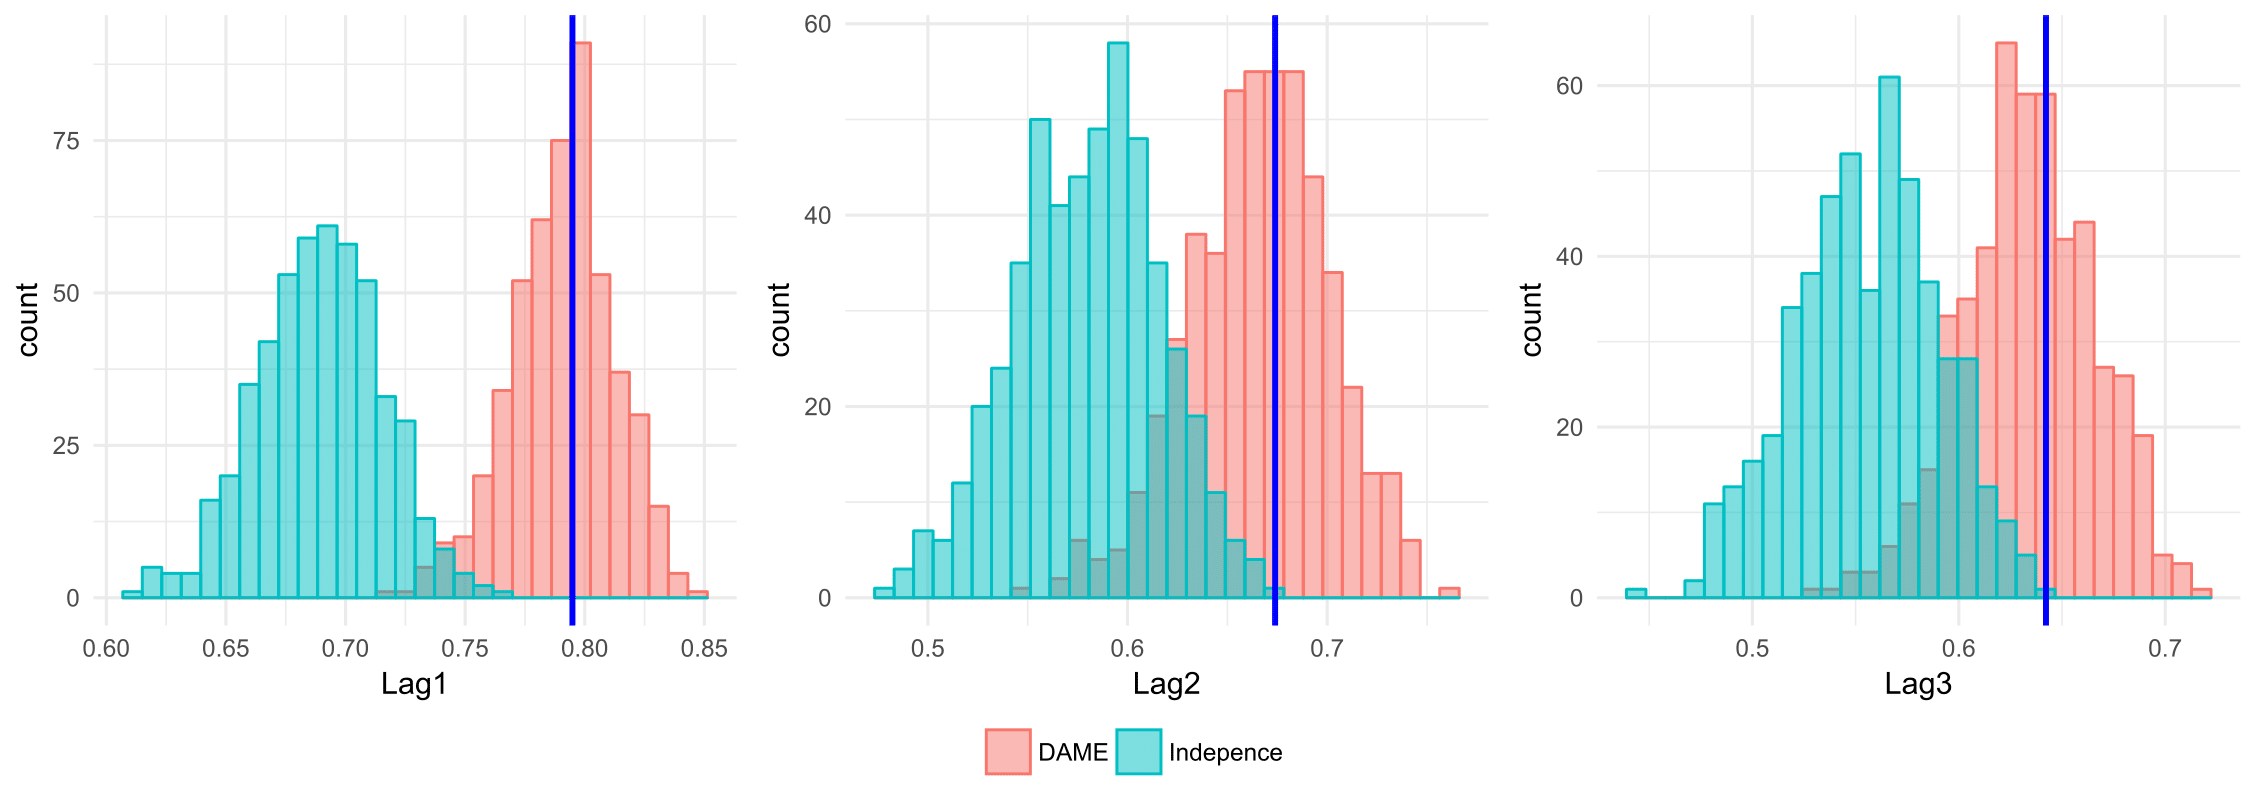
\includegraphics[width=1\textwidth]{plots_paper/correlations-1.png}	
	\caption {Histogram of posterior lagged degree correlations (from lag 1 to lag 3): the DAME (red) and independence model (green), with the observed dc statistic (blue lines).}
	\label{figure:correlationstudy}
\end{figure}
\subsection{Capturing Transitivity} \label{subsec: negative transitivity}
As introduced in Section \ref{sec: Introduction}, there exists two types of transitivities, positive and negative transitivity, and the parameterization of without $D$ term (i.e. $u^\prime u$) is not able to capture negative transitivity. To test if the DAME can explain both positive negative transitivities, we conducted another set of simulation study. Similar to Section \ref{subsec: correlation}, we generated  $\mathbf{Y}$ with $N=20$, $T=10$, $P=1$, $R=2$, and $\forall (a, b) = (2, 1)$. Considering that our new goal is not to estimate temporal correlations but to represent transitivity effect, this time we modify two settings: 1) set $(\kappa^\beta, \kappa^\theta, \kappa^d) = (0, 0, 0)$ such that all paramters and the resulting dynamic network is independent over time, and 2) fix $d^t_{r} = \pm 2$ for $r=1,2$ and $t=1,\ldots,10$ such that the generated network exibits positive, mixed, or negative transitive feature, respectively. Again, we ran 6,000 MCMC iterations and discarded the first 1,000 with thinning = 10, however, we fixed $\kappa$'s at the true values and did not estimate the covariance paramters (i.e. independence model) such that the difference in performance only comes from the multiplicative effects formulations---$u^\prime Du$ and $u^\prime u$. If we estimated $\kappa$'s for this comparison, the difference in results may not only arise from the formulation of multiplicative effects, but also possibly come from lack of correlation structure in $u^\prime u$ because our modeling framework do not assign any correlation on $u$'s.   \\ \newline 
Figure 2 shows a graphical comparison between the two formulations of the multiplicative random effects with respect to the first, second, and third moments of degree (i.e. degree($\hat{Y}$) degree($\hat{Y}^2$) and degree($\hat{Y}^3$), respectively), for a randomly chosen node. For the case of positive transitivity ($\forall d^t_{r} =+2$), our model and its alternative (without $D$ term) do not show significant differences; both formulations achieve great performance in replicating the first, second, and third moments of node 2's degree. On the contrary, when we fit the network with mixed ($\forall d^t_{r=1} =-2$ and $\forall d^t_{r=2} =+2$) or negative transitivity ($\forall d^t_{r} =-2$), the two formulations reveal noticeable differences. While the DAME can still recover the true degree in all three moments, the model without $D$ term shows inaccuracy in simulating a network that is close to the true data. Not only the $u^\prime u$ model introduces bias, but also it shows significanlty lower precision than our model. In addition, the evidence of $u^\prime u$ model's failure to estimate the transitivity statistics becomes larger as the network tends toward stronger negative transitivity and as we move to higher moments degrees. These findings strongly support our argument that $u^\prime Du$ should be preferred over $u^\prime u$, as a standard form of multiplicative random effects.
\begin{figure}
	\centering
			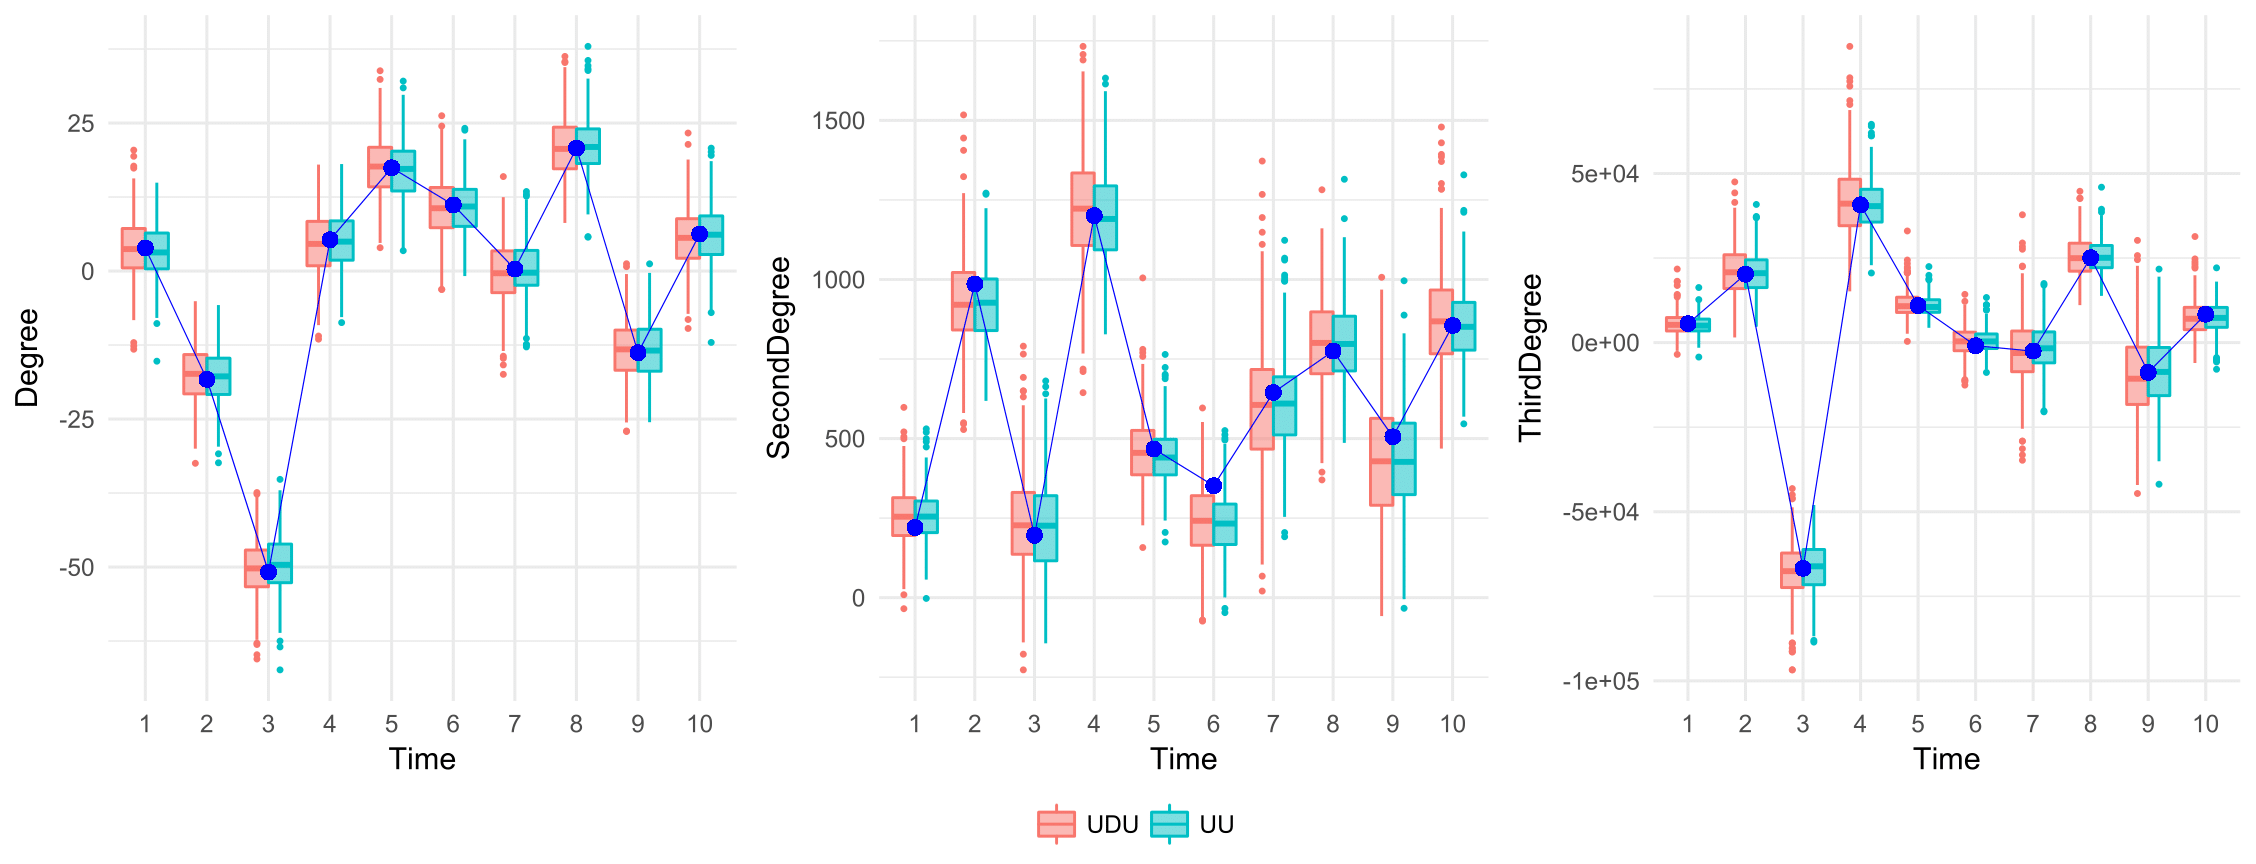
\includegraphics[width=1\textwidth]{plots_paper/newpositiveD-1.png}	
		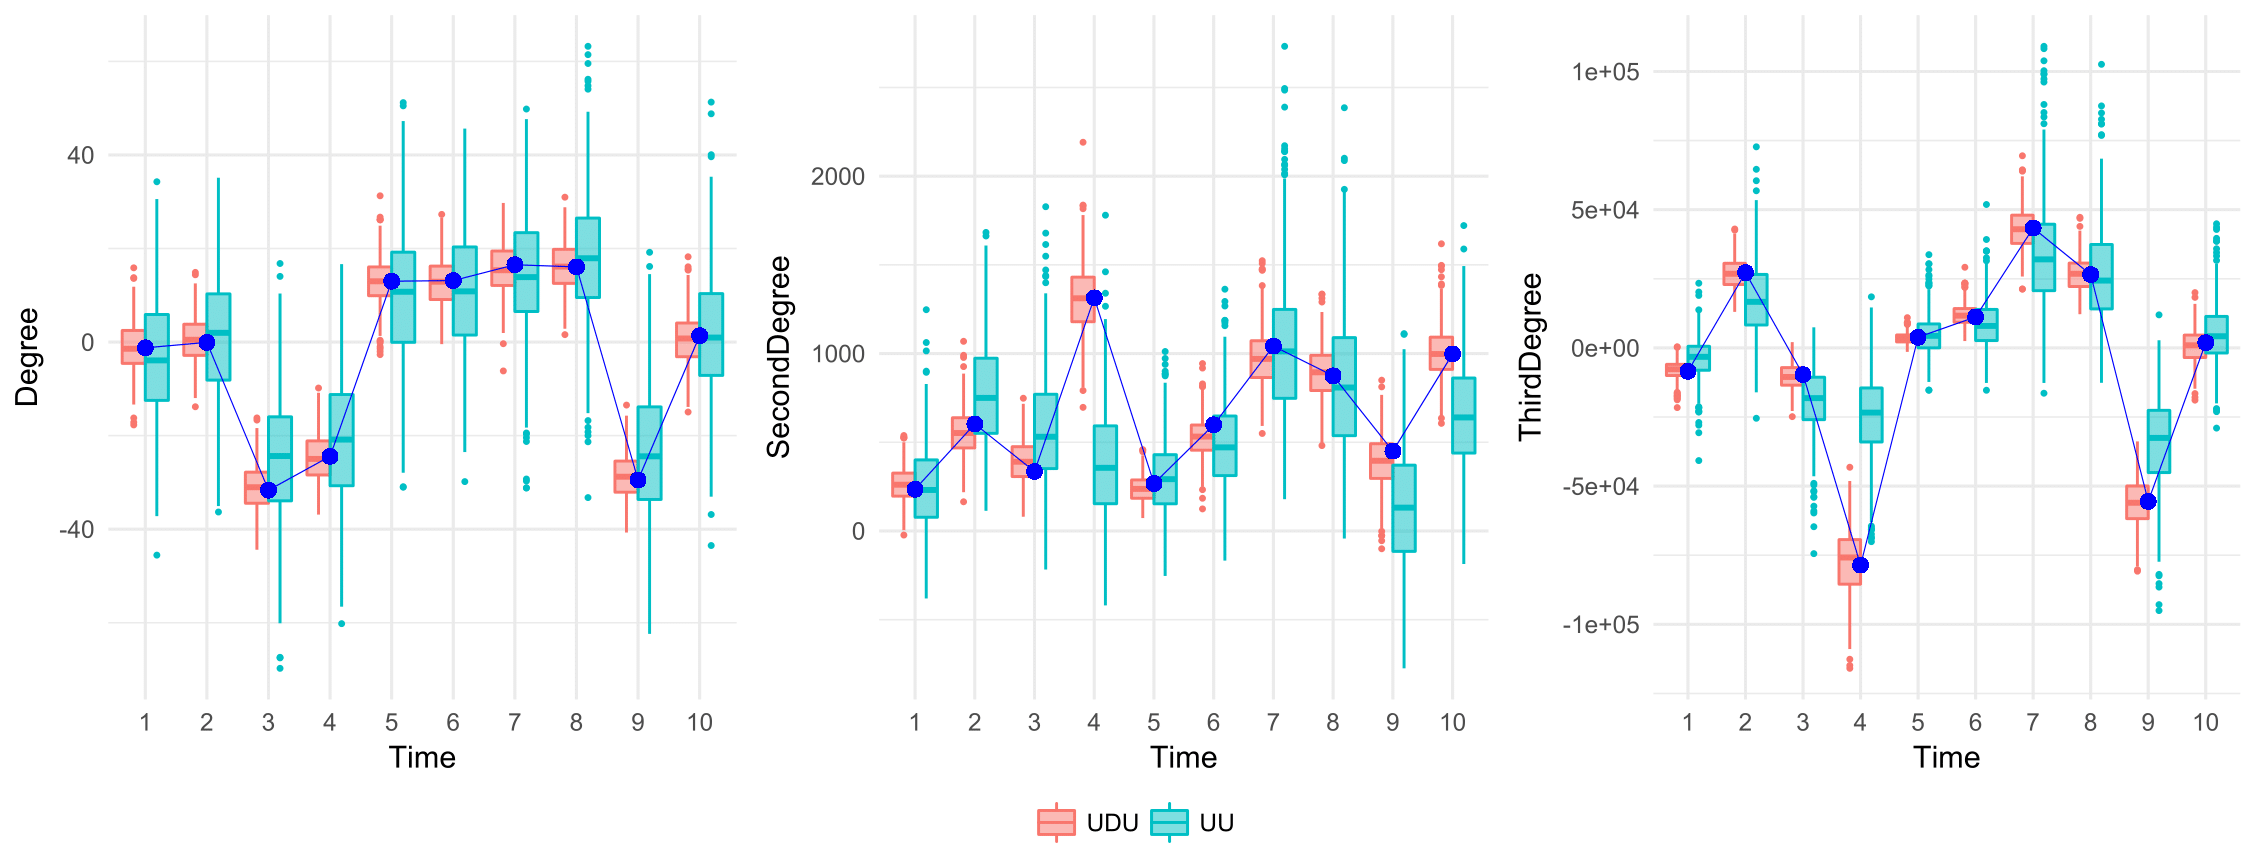
\includegraphics[width=1\textwidth]{plots_paper/newmixedD-1.png}	
						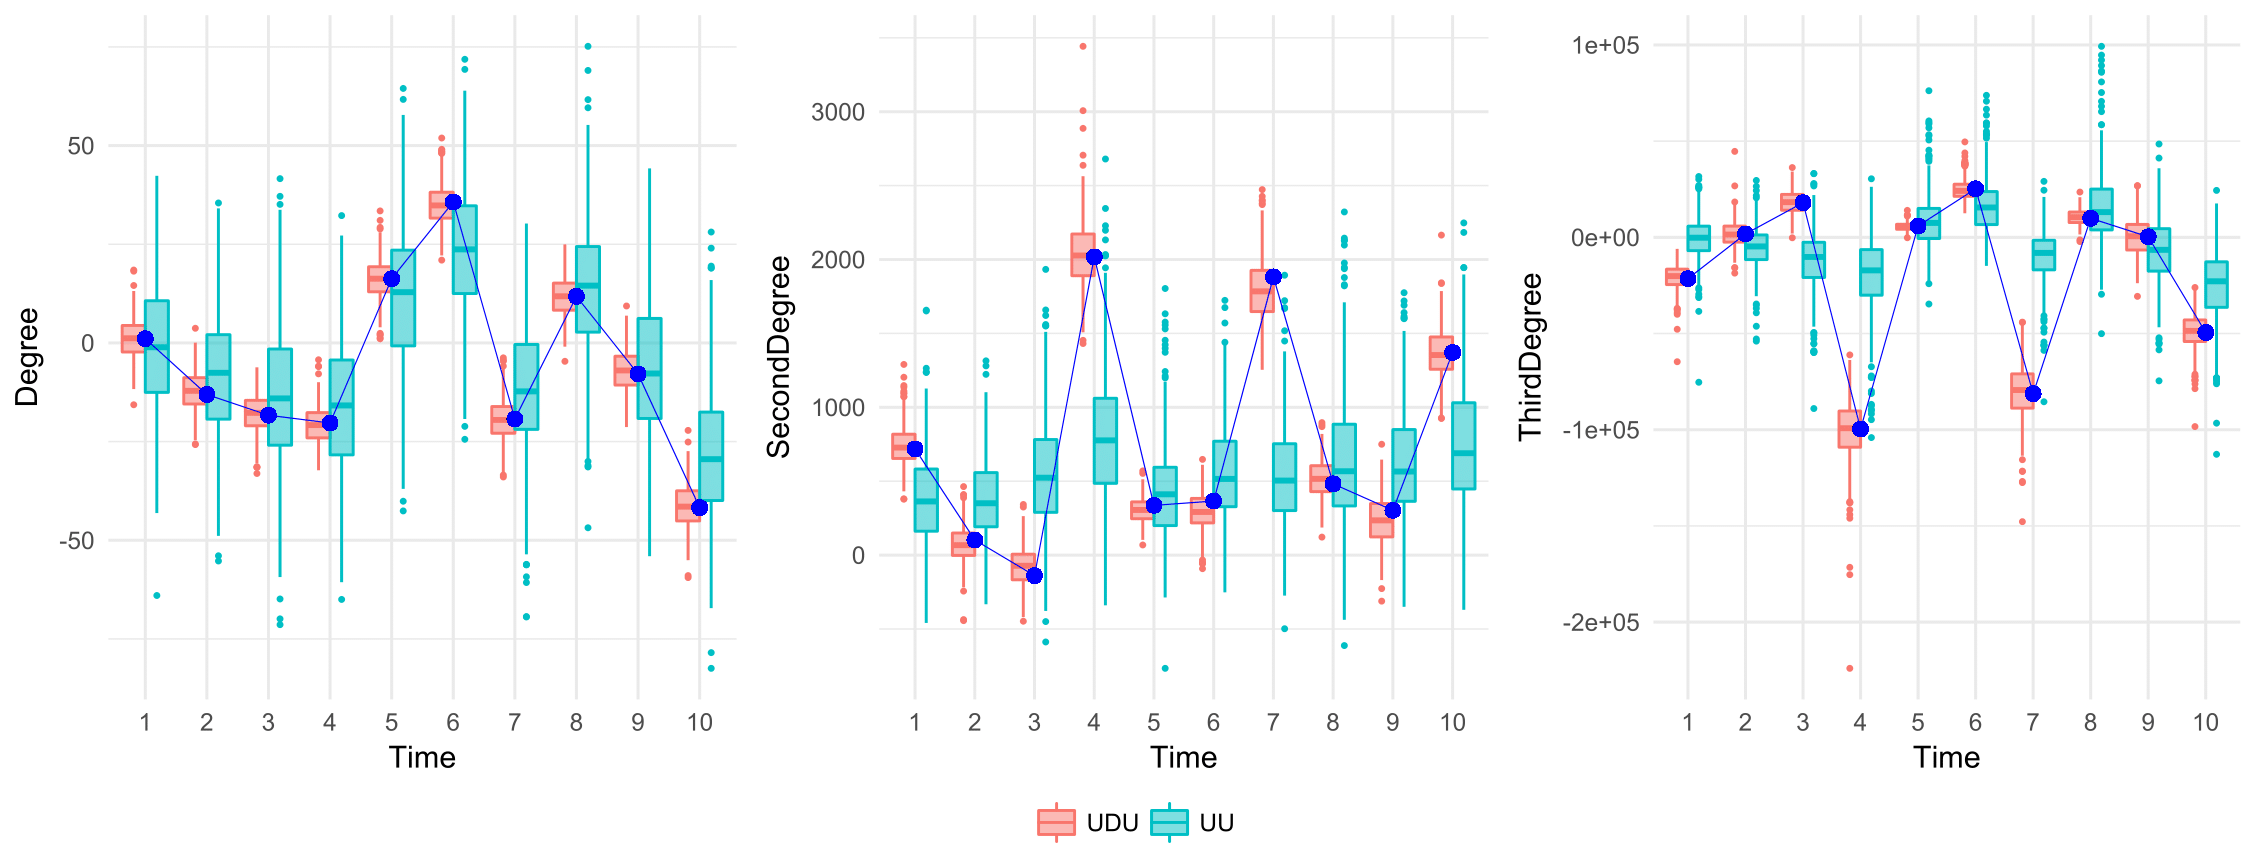
\includegraphics[width=1\textwidth]{plots_paper/newnegativeD-1.png}	
	\caption {Posterior distribution of the first (left), second (center), and third (right) moment degrees using positive transitive network (upper), mixed transitive network (middle), and negative transitive network (lower): the DAME (red) and $u^\prime u$ model (green), with the observed statistics (blue dots).}
	\label{figure:negativitystudy}
\end{figure}

\section{Analysis of the United Nations Voting Network}\label{sec: UNvoting}
\subsection{Data}\label{subsec: data processing}
Votes in the United Nations General Assembly (UNGA) have been analyzed in many political science papers \citep{voeten2000clashes,voeten2004resisting,bearce2007intergovernmental,mattes2015leadership,bailey2017estimating}, and became the standard data sources to measure the state preferences. The study of state preferences in international politics is one of the most important topics for students of international relations \citep{wendt_1994}. With regard to policy implications, for instance, states are the key actors at the global stage, knowing their preferences towards each other and tastes on difference issues, helps us predict future foreign policies and state behaviors. 
Unfortunately, the existing studies ignored three important features of the dataset. First, votes are highly correlated across timepoints, because they are the reflections from history. \cite{bailey2017estimating} proposed a dynamic ordinal spatial IRT (item response theory) model and allowed for better inter-temporal comparisons, however, their model limited the temporal dependence to be lag 1 (i.e. Markovian assumption---votes at time $(t+1)$ is only dependent on votes at time $t$). Second, although the researchers have viewed ``voting" as dyadic behavior and thus used dyadic similarity indicators such as affinity or S scores \citep{gartzke1998kant,signorino1999tau}, to our knowledge, the United Nations voting data has never been analyzed using the dynamic network models. Third, third-order dependence has not been modeled in the literature despite the fact that voting decisions are not limited to dyadic calculations---country A's decision to vote along the line with country B might well be influenced by a country C's decision. In order to overcome the limitations and provide the new insight at the same time, we apply the DAME to voting behavior in the United Nations General Assembly roll-call votes, from 1983 to 2014.\\ \newline
Here are the data processing procedures used in the analysis. First, the countries included in this analysis were determined by taking intersection of countries available for each variables (e.g. votes, polity score, GDP) and then dropping countries with missings (NA's) over 10 years, while the remaning missings were imputed using previous year's data. Full list of countries and their abbreiviations are listed in Table \ref{table:importantvotes} in Appendix \ref{appendix: countrylist}. Specifically, the voting data was obtained from \cite{12379_2016}, where we use the subset of the votes called `important votes', the votes identified as important by U.S. State Department report Voting Practices in the United Nations\footnote{For example, in 2001, important votes include `Israeli Actions in the Occupied Territories', `Peaceful Settlement of the Question of Palestine', `U.S. Embargo Against Cuba', and `Nuclear Disarmament'.}. We did not include all votes from the original data in that non-important votes may not strongly reflect state preference of the countries. Throughout 1983 to 2014, the number of important votes on average is 12 per year, ranges from 6 to 28. We constructed the response $\mathbf{Y} = \{Y^1,\ldots, Y^{32}\}$, where each $Y^t$ is $97\times 97$ matrix, using the variable `agree3unimportant' in the original dataset, which is a voting similarity index (0--1) computed using 3 category vote data (Y = “yes” or approval for an issue; A = abstain; N = “no” or disapproval for an issue)\footnote{Voting similarity index between the two countries $i$ and $j$ at year $t$ is calculated as (Number of votes $i$ and $j$ agreed at year $t$) / (Number of votes $i$ and $j$ both participated at year $t$)}. Note that abstention is counted as half-agreement with a yes or no vote \citep*{12379_2016}, while two abstention is treated as full-agreement. For basic summary of Unite Nations voting data including the average number of common votes and the averge proportion of agreement or voting similarity index per year, see Table \ref{table:EDA} in Appendix \ref{appendix: summarystat}. \\ \newline
As an exploratory data analysis, Table \ref{table:corr} illustrates the lagged degree correlation (defined in Equation \ref{eqn:dc}) of the observed dataset to measure how strong Unite Nations voting data is correlated over time. There exists strong positive correlation in how countries vote in the United Nations General Assembly over time, and as the distance between two timepoints become larger the correlation gets weaker. This provides solid evidence that our model with Gaussian process assumption is one of the appropriate appraoches to account for strong temporal dependence in the dataset.
\begin{table}[ht]
	\centering
	\begin{tabular}{ |c|c|c|c|c|c|c|c|c|c|c|} 
		\hline
		{Lag}	& 1 & 2& 3& 4& 5& 6& 7&8&9&10 \\ \hline
		dc & 0.732&0.623&0.513&0.435&0.395&0.315&0.263&0.158&0.164& 0.203\\\hline
	\end{tabular}
	\caption {Lagged degree correlation of United Nations Voting Data for Lag 1 to 10.}
	\label{table:corr}
\end{table}
\newline Next, to dynamically model the voting network in relation to other variables reflecting international relations, we combine $P=5$ different dyadic variables from the Correlates of War (COW) data \citep{gibler2008international}, Polity IV data \citep{marshall2014polity} and the International Monetary Fund (IMF)'s Direction of Trade Statistics (DOTS) and International Financial Statistics (IFS) data, and construct the observed edge covariates $\mathbf{X}$. For every $p=1,\ldots,5$, we set the explanatory variable $X^t_{ijp}$ as below.
\begin{itemize}
	\item [1.] $\mbox{Intercept}^t_{ij}$: constant 1,
	\item [2.] log($\mbox{distance})^t_{ij}$: log of the geographic distance between country $i$ and country $j$,
	\item [3.] $\mbox{Alliance}^t_{ij}$: 1 if country $i$ and country $j$ have alliance, and 0 otherwise,
	\item [4.] $\mbox{Polity difference}^t_{ij}$: absolute difference in polity IV number between country $i$ and country $j$,
	\item [5.] $\mbox{Lower trade-to-GDP ratio}^t_{ij}$: index of economic dependence using bilateral trade weighted by each country's gross domestic product (GDP), as defined in \cite{gartzke2000preferences} $$min\Big(\frac{\mbox{Trade}_{ijt}}{\mbox{GDP}_{it}}, \frac{\mbox{Trade}_{ijt}}{\mbox{GDP}_{jt}}\Big),$$
	\item [6.] $\mbox{Common language}^t_{ij}$: indicator of whether country $i$ and country $j$ share the same language,
\end{itemize}
where all covariates are symmetric $X^t_{ijp}=X^t_{jip}$. Note that intercept is included to account for the baseline degree of agreement at each timepoint. Two variables, log($\mbox{distance}$) and common language are time-invariant covariates, although their coefficients may vary over time. Correlations between the five covariates (except the intercept) are attached in Appendix \ref{appendix: correlations}.\\\newline
Moreover, we specified the matrix of availability $A$ introduced in Section \ref{subsec: varying number of nodes} to reflect six countries' nonparticipation in the United Nations Genearl Assembly: 
\begin{itemize}
	\item[1.]  North Korea (PRK) have structural zeros from $t = 1$ to $t = 8$:\\
	- North Korea did not vote until North Korea and South Korea have simultaneously admitted to United Nations in 1991.
	\item[2.] South Korea (ROK) have structural zeros from $t = 1$ to $t = 8$:\\
	- South Korea did not vote until North Korea and South Korea have simultaneously admitted to United Nations in 1991.
	\item [3.] Russia (RUS) has structural zeros from $t=1$ to $t =9$:\\
- Russia succeeded the Soviet Union's seat, including its permanent membership on the Security Council in the United Nations after the dissolution of the Soviet Union in 1991. 
	\item [4.] Iraq (IRQ) has structural zeros from $t =13$ to $t = 21$:\\
	- The country did not participate the UNGA roll-call votes during 1995--2003. Under the rule of Saddam, Iraq was under severe sanctions from the international community including the United Nations since 1990.
\end{itemize}
Therefore, any missing values corresponding the country and missing period are treated as structural zeros. As in Section \ref{subsec: varying number of nodes}, other non-structural missing values are treated as random missing (and thus imputed). 
\subsection{Reduced-Rank Structure of Voting Network}\label{subsec: reduced rank}
In this section, we demonstrate the special low-rank structure of the voting network, which can be generalized into any other similarly constructed agreement networks. First, for simplicity, we assume static network by fixing $T = 1$ and consider the $N \times N$ adjacency matrix $V^1$ representing the network consists of single vote. Since each entry of $V^1$ denotes a voting similarity index (0-1) computed using 3 categories (“yes”, ``abstain", and “no”), the $(i, j)^{th}$ element $V^1_{ij}$ can only have three possible values,
\begin{equation*}
V^1_{ij} =\begin{cases}
1, & \mbox{agreement}\\
0.5, &\mbox{half-agreement (one abstain)}\\
0, & \mbox{disagreement}\\
\end{cases}
\end{equation*}
which implies perfect transitivity of the agreement network, i.e. if there is an agreement between $i$ and $j$, and also between $j$ and $h$, then there must be an agreement between $i$ to $h$, and therefore any two edges sharing one node, such as $V^1_{ij}$ and $V^1_{jh}$, automatically determines the third edge between the unshared nodes $V^1_{ih}$. This constraint makes the maximum rank of $V^1$ to be 3, thus we can use low rank factorization of the matrix $V^1$ using $R=3$. If we were to apply the DAME model to this type of single vote network (without additive effects and explanatory variables), the maximum size of dimension for the latent factors we could fit is $R=3$ and the estimated latent factors can be viewed as the distinct constructs behind the vote. \\ \newline
\iffalse When two votes are aggregated, following the theorem regarding the bounds on the rank of the sum of matrices (modified for symmetric matrices) \citep{marsaglia1967bounds}
\begin{equation*}
 r(A + B) \leq r(A) + r(B) - \mbox{max}(d), 
\end{equation*}
where $r(A)$ is the rank of matrix $A$ and $d = \mbox{dim}(\mathcal{C}_A \cap \mathcal{C}_B)$ with $\mathcal{C}_A$ denoting the column space of $A$, the maximum rank of the matrix $V_1+V_2$ becomes 6. \textcolor{red}{However, due to the perfect transitive constraint of agreement network, $\mbox{max}(d)$ is always greater than 0, thus the maximum rank is 5 in our case.} As a result, we can generalize this finding into the aggregate of $M$ votes:
\begin{equation*}
\mbox{The maximum rank of the matrix $(V_1+V_2,\ldots,V_M)$ is $3 + 2\times (M-1)$,}
\end{equation*}
which is the maximum dimension of latent factors the DAME model could fit, although small value of $R$ (e.g. $R=2$ or $3$) are preferred in general. \fi 
Although it is worth understanding the constraint behind single votes, this is not a practical issue in modeling United Nations voting network, where we aggregate multiple votes per year (minimum number of important votes per year is 6). When we add $M$ number of matrices representing each vote, the aggregated matrix $V^1+V^2+...+V^M$ gets closer to the full rank thus we no longer need to concern about the maximum dimension of the latent factors in fitting the DAME model. Moreover, including the observed covariates $\mathbf{X}$ and additive random effects $\theta$'s also relax the reduced rank structure, since the multiplicative latent effect $u^\prime Du$ is modeled after we subtract those effects from the response matrix or array (See Section \ref{sec: DAME}). Accounting for large variability in the observed covariates and additive random effects, the residuals no longer maintain the perfect transivity structure.
\subsection{Model Validation}\label{subsec: Model Validation}
We perform a model validation to check if the DAME is an accurate and credible model for the data and to understand the role of different effects at the same time. We fitted four different dynamic AME models, one with additive and multiplicative effects (DAME), one with only multiplicative effects (ME), one with only additive effects (AE), and the last without any random effects (NO), where all four models included 6 fixed effects in Section \ref{subsec: data processing}. We constructed 95\% credible intervals of the degree statistics constructed from the model-simulated response $\hat{\mathbf{Y}}$ from the four separate models. \\ \newline
Figure \ref{figure:modelvalidation} shows the comparison of posterior degree distributions of the country ``Israel". First of all, there is huge benefit of correcting the bias when we add additive effects, compared to the model with no random effects. Next, when we compare between AE and ME, it is noticeable that the multiplicative effects significantly reduced the interval of estimates. This happens since the additive effects have very small variances while the multiplicative effects have larger variance estimates, which significantly lowered the error variance estimates $\hat\sigma_e^2$ that plays a big role in the precision of simulated data. Our model with both additive and multiplicative effects (DAME) seems to perform similar to the ME model in this plot, however, further analysis showed that the DAME still outperform the ME model in terms of both accuracy and precision. Overall, not only the DAME model showed the most accurate estimates over time, but it also had the narrowest 95\% credible intervals among the four. These findings emphasize the importance of including the additive and multiplicative term which enable the model to capture some features not explicable by fixed effects and maximize the model performance. More results and interpretation using the full DAME model are demonstrated in Section \ref{subsec: UNresult}, and the posterior predictive plots checking the overall degree distributions (aggregate all nodes and timepoints) can be found in Appendix \ref{appendix: PPC}.
\begin{figure}[H]
	\begin{center}
		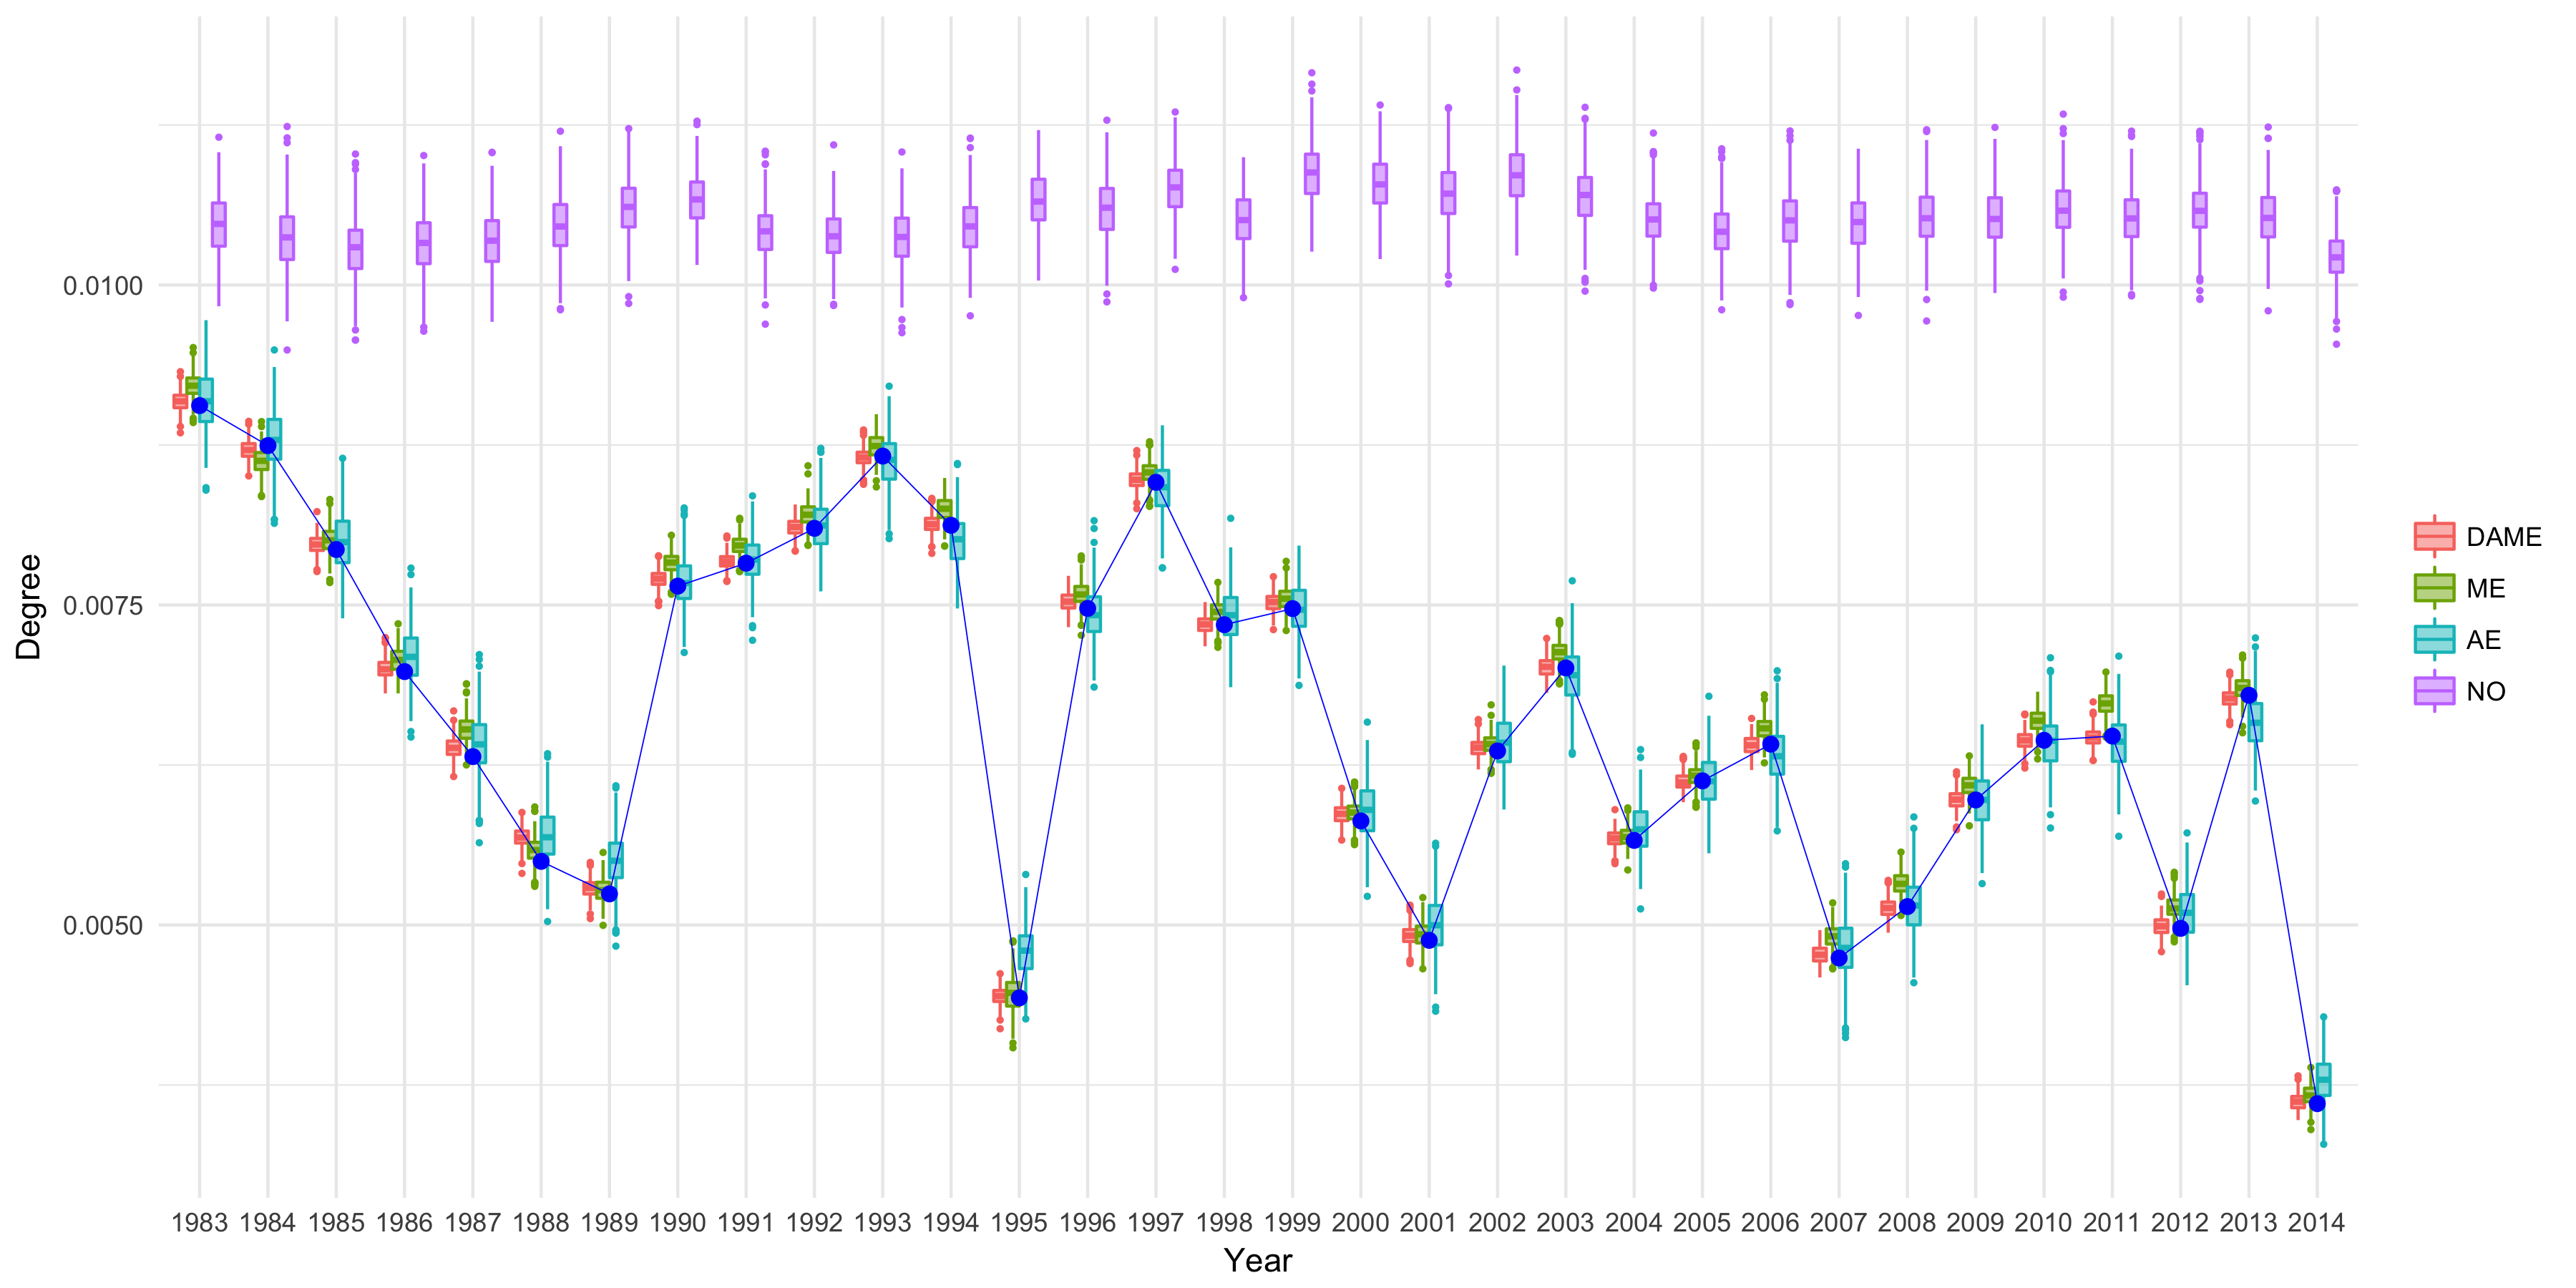
\includegraphics[width=1\textwidth]{plots_paper/ISR79.png}	
	\end{center}
	\caption {95\% credible intervals for posterior degree of Israel (ISR), comparing four models: the DAME (red), only multiplicative effects (green), only additive effects (blue), and no random effects (blue), with the blue dots represent the country's observed degree statistics.}
	\label{figure:modelvalidation}
\end{figure}
\subsection{Parameter Estimation and Interpretation}\label{subsec: UNresult}
In this section, we apply the model with the dimension of latent factors chosen as $R=2$, based on some preliminary experiments where increasing the dimension of latent factors did not significantly improve the model fitting. For example, when $R=3$, the last value of estimated eigenvalue $d_{3\cdot}$ is very close to zero for the most of the timepoints $t=1,\ldots,32$. Thus, we present the results from the same settings as Section \ref{subsec: Model Validation}, which are $30,000$ Gibbs iterations with a burn-in of $5,000$, where every $50^{th}$ sample was taken as a thinning. All inverse-Gamma hyperparameters $(a, b) = (2, 1)$, and the covariance parameters $(\kappa, \tau)$ were estimated, following Section \ref{subsec: posterior computation}. Figure \ref{figure:interceptplot} shows the posterior mean estimates of the fixed effect coefficients $\{\beta_p\}_{p=1}^6$ with their corresponding 95\% credible intervals. \textcolor{red}{Interpretation of fixed effect plot} \\
\begin{figure}[ht]
	\begin{center}
		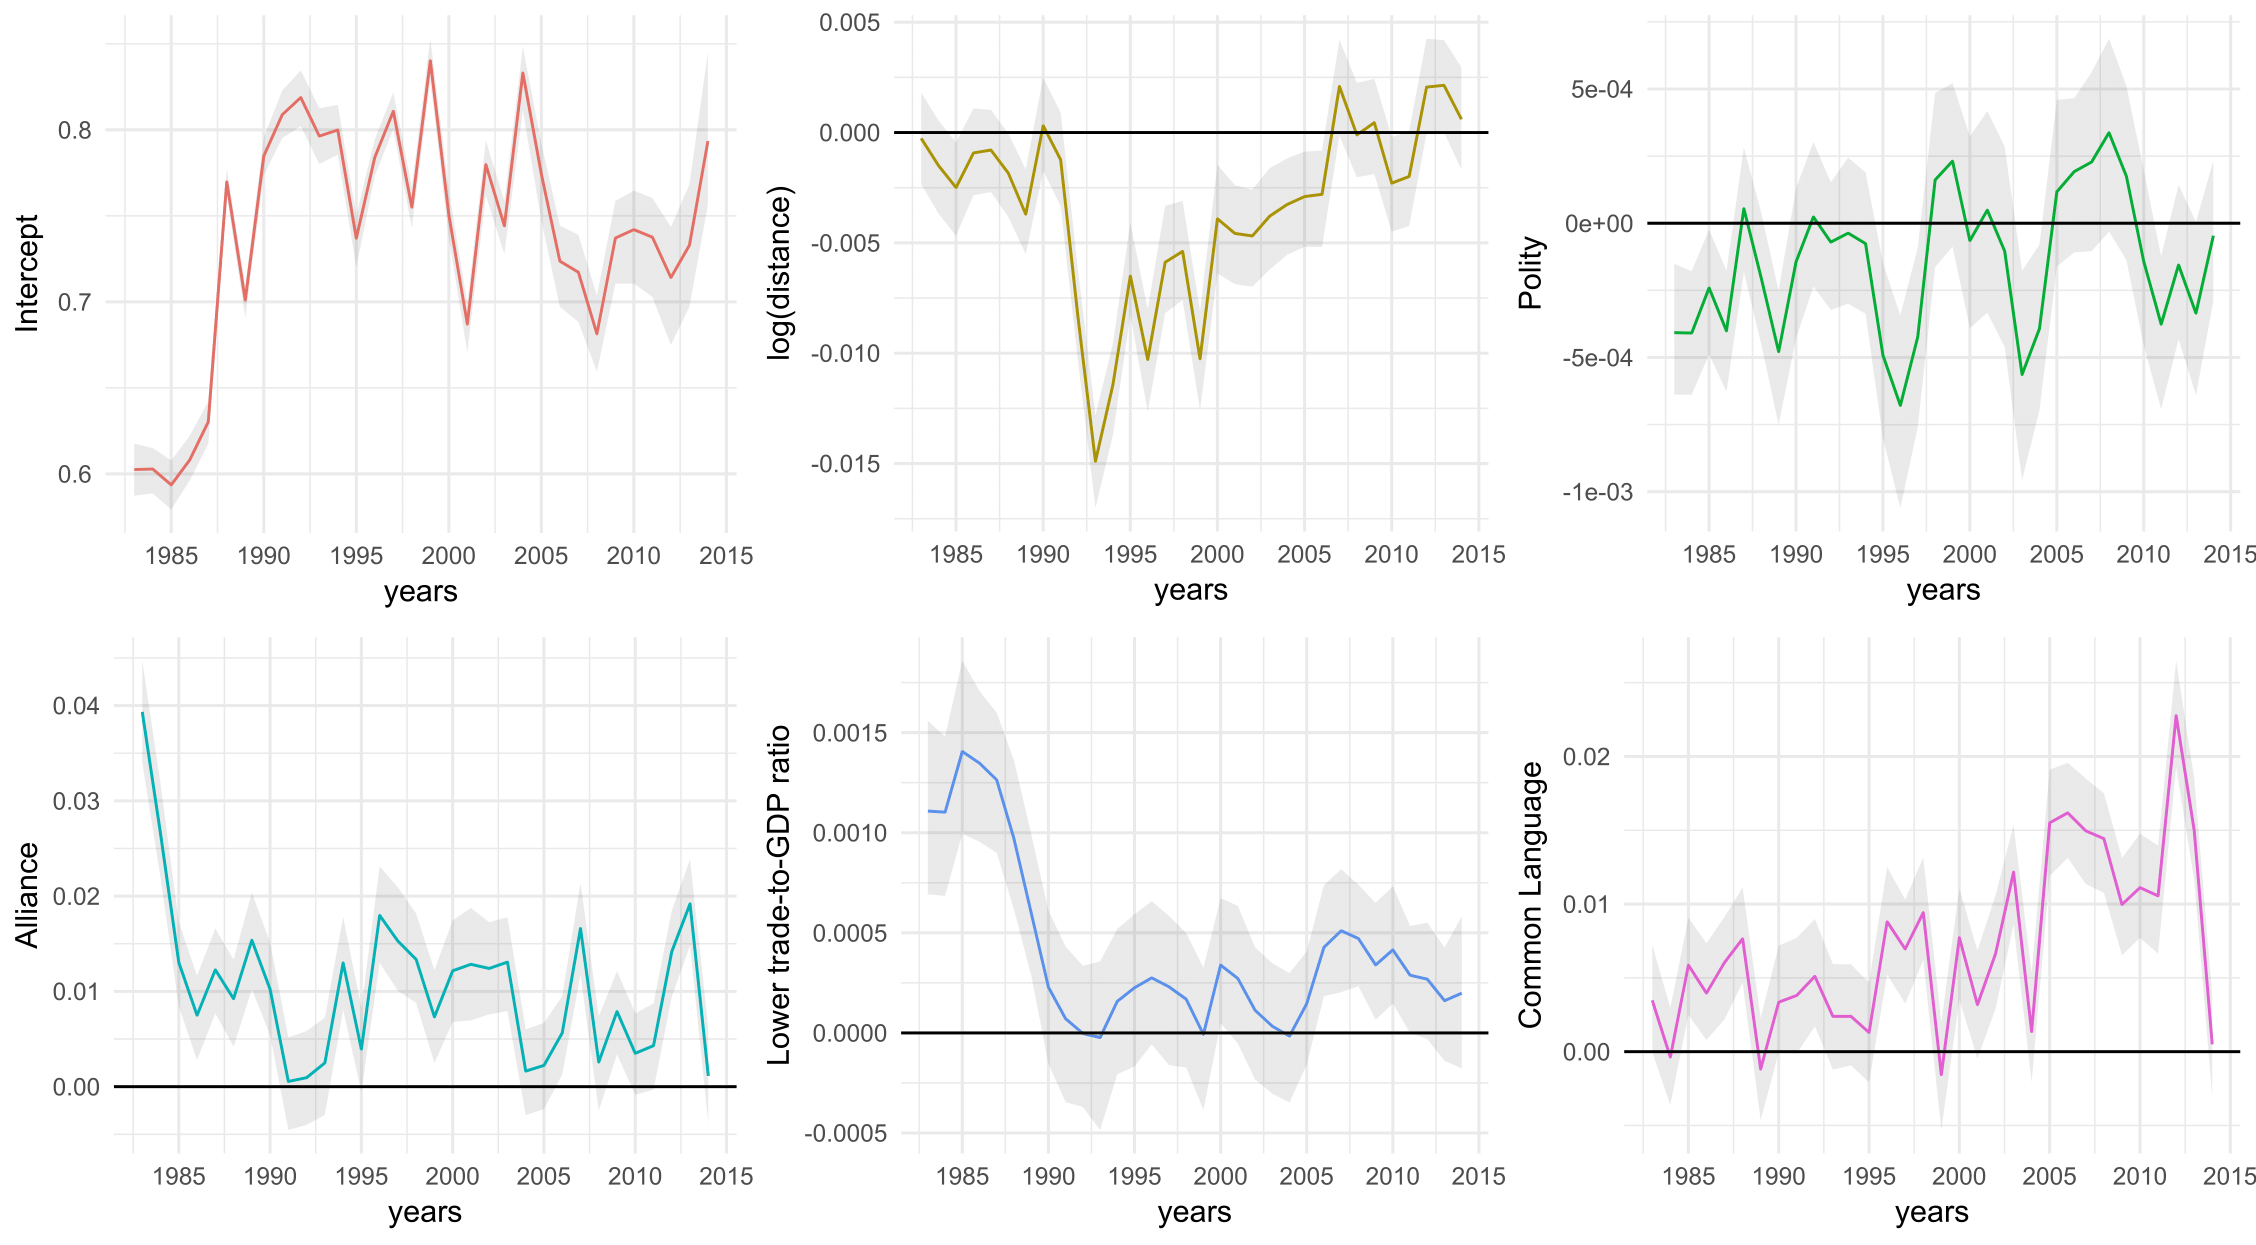
\includegraphics[width=1\textwidth]{plots_paper/betaplot-1.png}
	\end{center}
	 	\caption {Posterior mean for the fixed effect coefficients $\{\beta_p\}_{p=1}^6$  (colored line): Intercept, log(distance), Alliance, Polity difference, Lower trade-to-GDP ratio, and Common Language, and their corresponding 95\% credible intervals (grey areas). }
	\label{figure:interceptplot}
\end{figure}
 \begin{figure}[ht]
 	\begin{center}
 		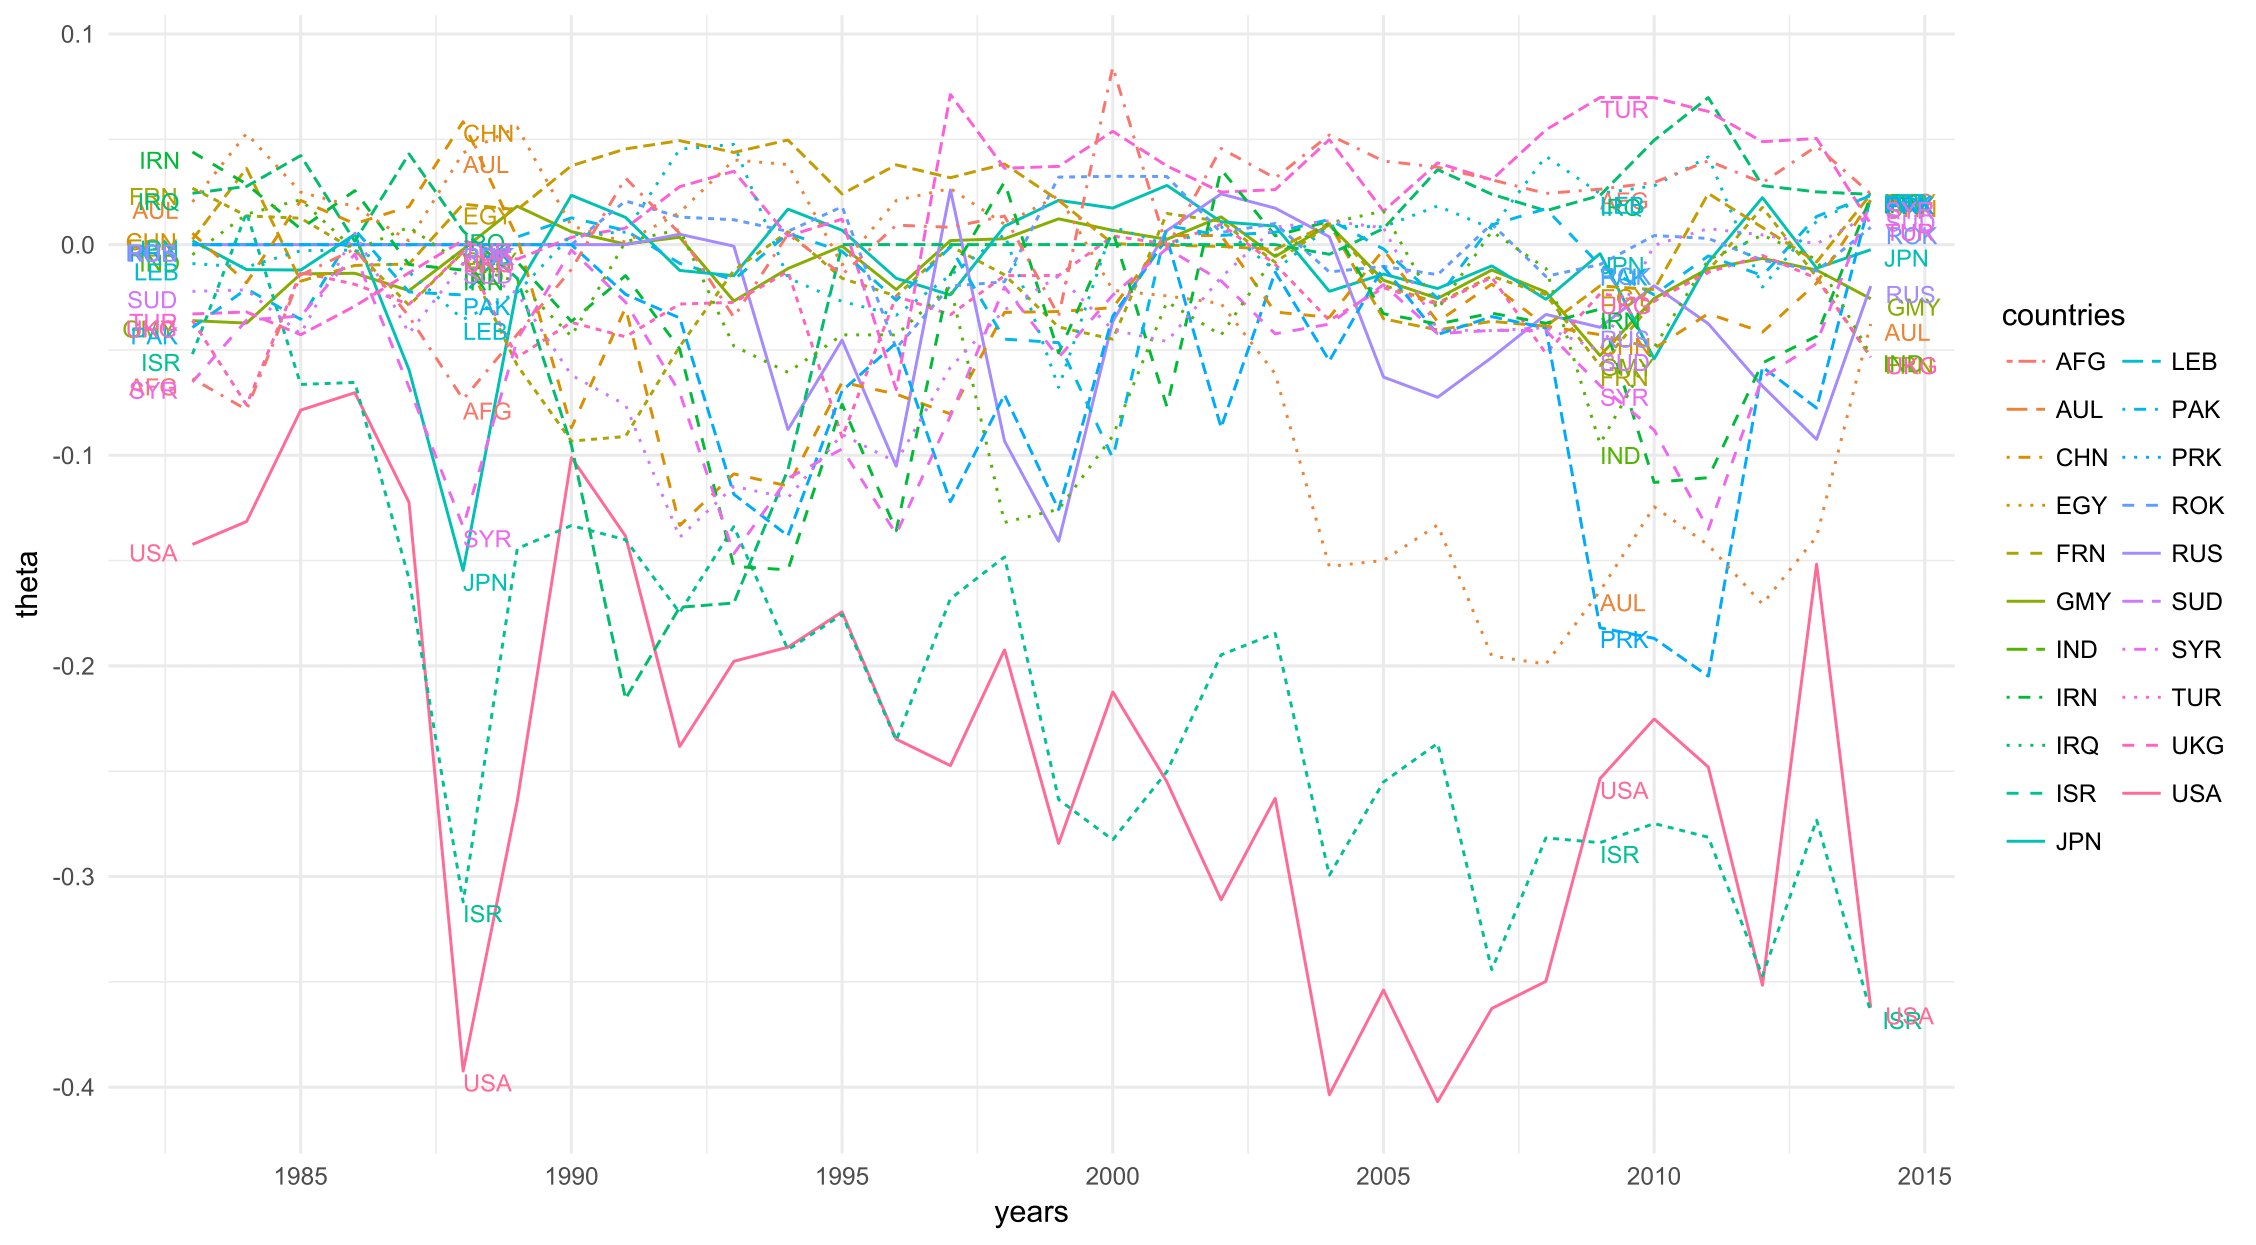
\includegraphics[width=1\textwidth]{plots_paper/thetaplot-1.png}	
 	\end{center}
 	\caption {Posterior mean estimates for the additive random effect estimates $\theta$.}
 	\label{figure:thetaplot}
 \end{figure}
 \newline\noindent After controlling for the observed covariates, we move on to the analysis of random effects, both additive and multiplicative ones. For clear visualization, we only present the results from 21 countries, where the countries are chosen based on the most active countries during the ten year period of 2004 -- 2014 \citep{hoff2015multilinear}. Here, the action types include negative material actions, positive material actions, negative verbal actions and positive verbal actions. The 21 countries are marked with $*$ in Appendix \ref{appendix: countrylist}. Figure \ref{figure:thetaplot} is the posterior mean estimates of each node or country's additive random effects which capture the node-specific and within-dyad dependence. \textcolor{red}{Interpretation of additive random effects}\\ \newpage
\noindent The estimated latent factor coordinates in Figure \ref{figure:UDplot}, which can be viewed as the latent positions of the nodes, demonstrate the remaining higher-order network dependencies in United Nations voting behaviors. To determine the posterior estimates of $u$ without identifiability issue, we applied eigen-decomposition on every posterior sample of the multiplicative effect matrix $u^\prime Du$, and let $D$ be the diagonal matrix of $R$-number of eigenvalues and $u$ be the corresponding eigenvectors. For Figure \ref{figure:UDplot}, we applied Procrustes transformation on each posterior estimate of $u$ and multplied $\sqrt{d}$, and then obtained the 95\% confidence regions. \textcolor{red}{Interpretations --- What shoud be said about this multiplicative effect plots?} \\ \newline As illustrated, the model estimated additive and multiplicative latent effects and the movement of latent positions reveal that United Nations voting network reflects interesting and meaningful foreign policy positions and alliance of various countries, even after controlling for other covariates that are considered critical in the international relation studies.
  \begin{figure}[ht]
  	\begin{center}  
  		 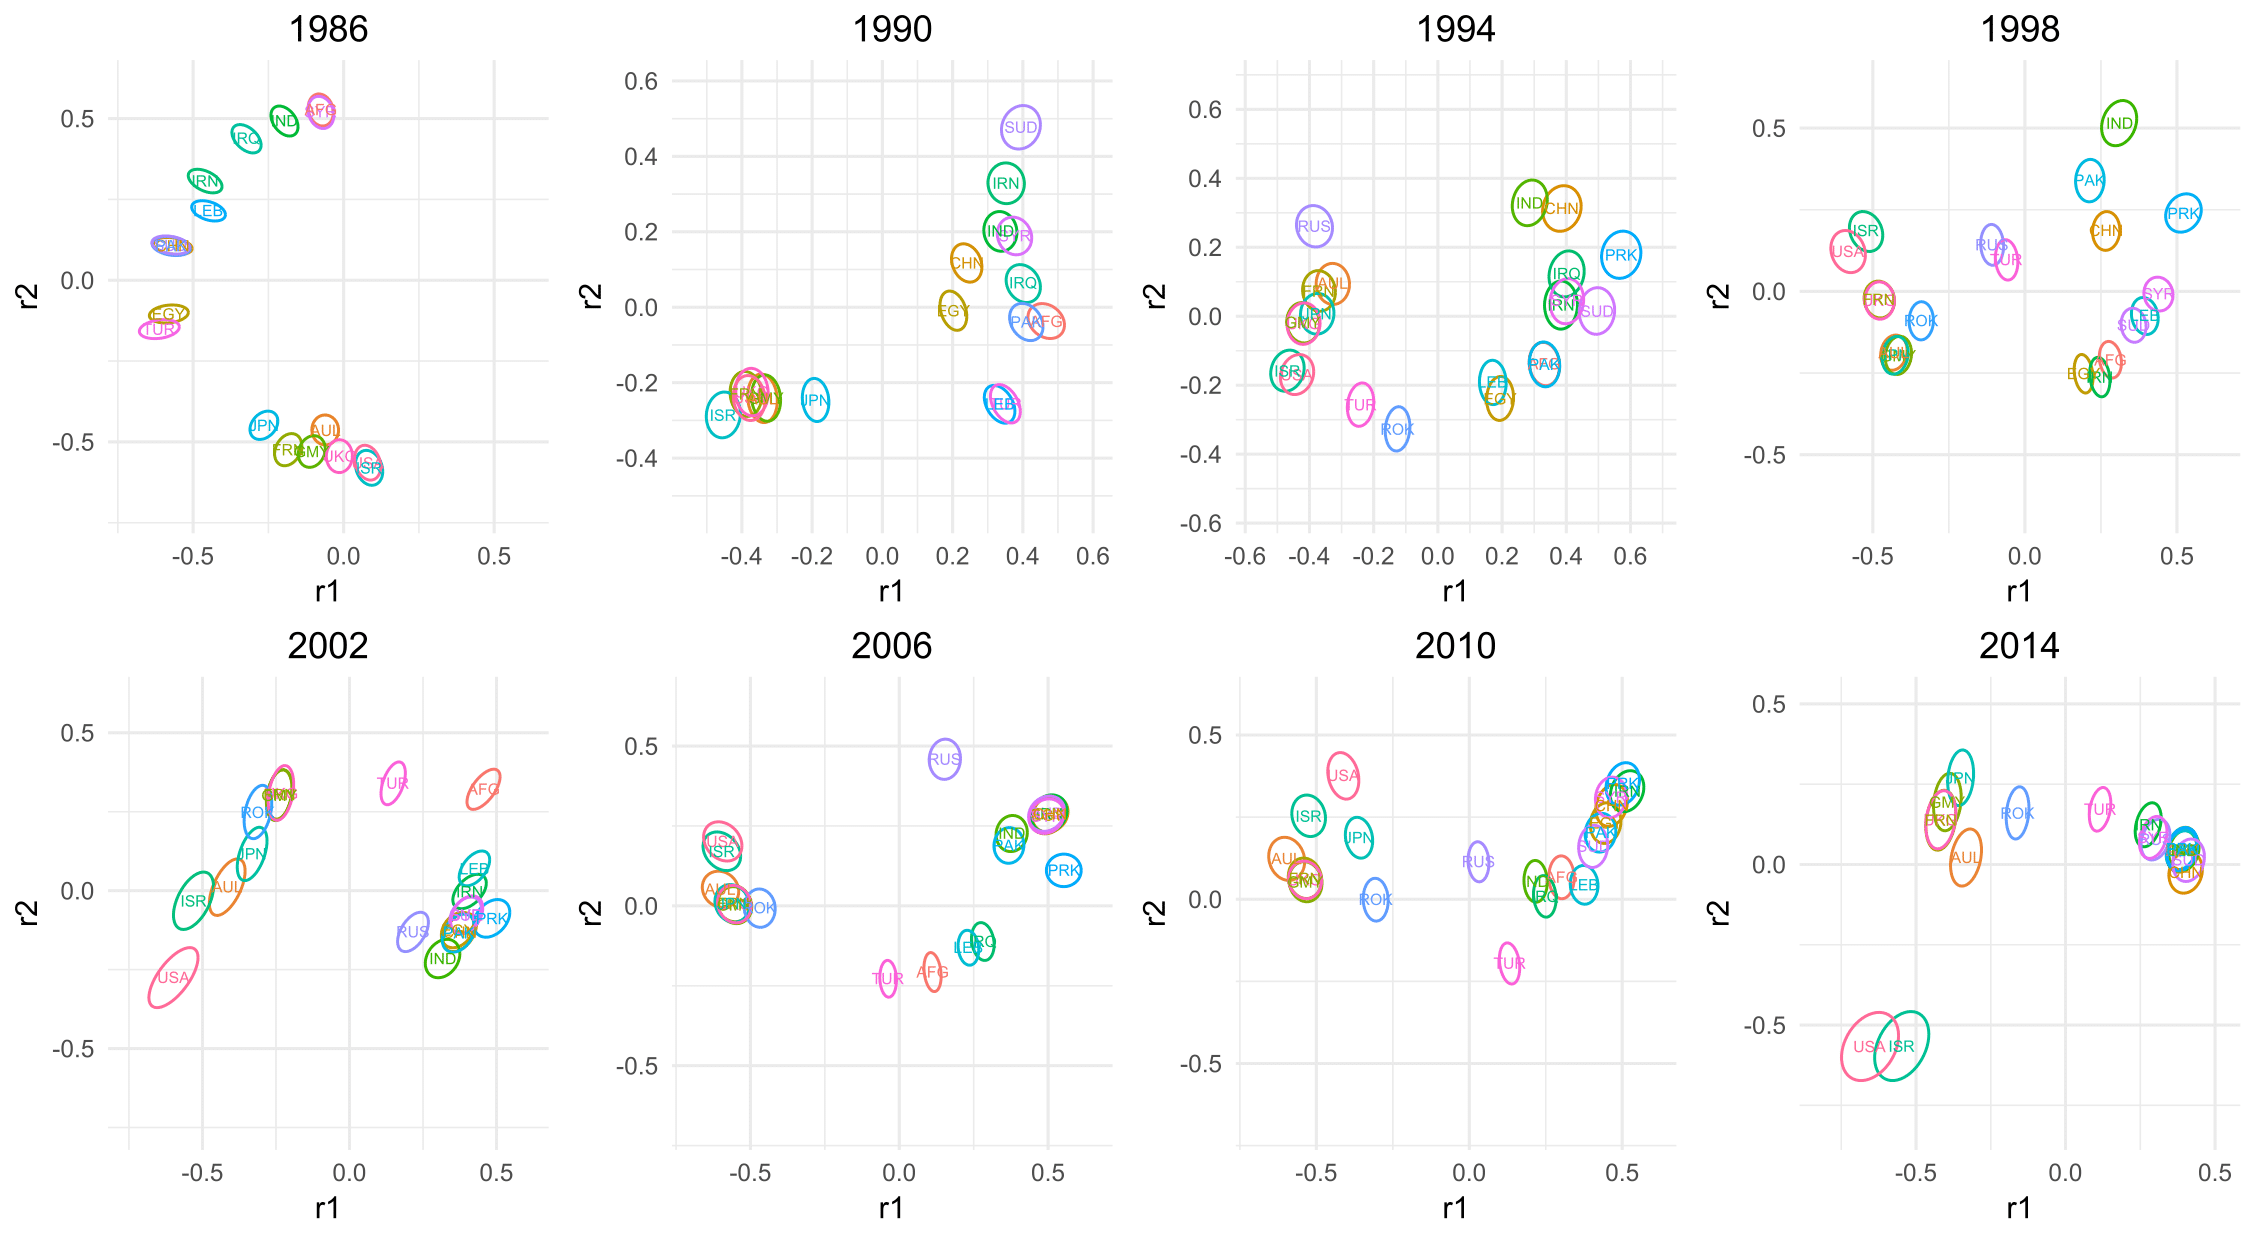
\includegraphics[width=1\textwidth]{plots_paper/UDU_reduced_8years-1.png}
  	\end{center}
  	\caption {Posterior mean estimates for the multiplicative random effects and their corresponding 95\% credible regions for the 21 selected countries for every 4 years between 1983 and 2014.  }
  	\label{figure:UDplot}
  \end{figure}
  \newpage
\section{Discussion}
Using the correlation associated with network at each time point makes better use of dynamic networks than modeling them as a separate network snapshots. Our algorithm eliminates the need to make an arbitrary user-defined covariance structure for determining the prior on the parameters, making it easier to understand the temporal dependence from the data which is  highly informative and also lead to more accurate inference.  As a time-varying coefficient extension of the additive and multiplicative effects (AME) model, the dynamic additive and multiplicative nework effects (DAME) model can flexibly learn time-varying network structures, while inferring the effects of latent variables. Further, the visualization of the model estimated time-varying parameters provides an effective temporal trend analysis of dynamic networks, as well as the descriptive visualization of higher-order dependencies from the latent positions over time.
\\\newline
We have demonstrated such effectiveness of our model by modeling the United Nations Voting networks. Although we illustrated the entire framework in the context of symmetric or undirected networks, our model can be easily extended to allow directed networks, following the specification of additive and multiplicative effects model for the directed network \citep{minhas2016inferential}. Furthermore, the approach can be applied to binary and ordinal network data with appropriate link functions, while we currently only provide the application to continuous-valued networks.  Finally, considering the recent explosion of network dataset with extremely large number of nodes or timepoints, our model has a broad range of applicability, suggesting promising computational methods that can accommodate huge networks.
\bibliographystyle{apalike}
\bibliography{BominBib2}
\newpage
\begin{appendices}
\section{List of Countries in Voting Network}\label{appendix: countrylist}
\begin{table}[H]
	\centering
\begin{tabular}{c|c||c|c}
	\hline
	Abbreviation&Country or area name &	Abbreviation&Country or area name\\
	\hline
			AFG* & Afghanistan & 	KUW & Kuwait\\
				ALB & Albania & LEB* & Lebanon\\
			ALG & Algeria & LIB &Libya \\
		ANG & Angola 	& MAA&  Mauritania\\
		ARG& Argentina	&MEX &Mexico \\
		AUL* & Australia&MLI&Mali\\
		BAH & Bahrain	&MOR & Morocco\\
	BEN & Benin 	&MZM & Mozambique\\
			BFO & Burkina Faso 	&NEW & New Zealand \\
	BNG&  Bangladesh	& NIC& Nicaragua\\
			BOL& Bolivia	& NIG &      Nigeria\\
		BRA &Brazil&NIR & Niger\\
				BUI & Burundi &NOR &Norway \\
		BUL & Bulgaria	&NTH &  Netherlands\\
		CAN & Canada	& OMA & Oman\\
		CAO & Cameroon	&PAK* & Pakistan\\
		CEN & Central African Republic	&PAN & Panama\\
			CHL & Chile &PAR & Paraguay\\
			CHN* & China	& PER & Peru \\
		COL & Colombia	&PHI & Philippines\\
			CON & Congo		&POL & Poland\\
			COS & Costa Rica&POR & Portugal\\
			DEN& Denmark	 & PRK* & North Korea\\
			DOM & Dominican Republic	&QAT & Qatar\\
		ECU &Ecuador 	&ROK* & South Korea\\
			EGY* & Egypt	&RUS* & Russia\\
				FIN & Finland	&RWA & Rwanda\\
			FRN* & France&SAL & El Salvador\\
			GAB & Gabon 	&SAU & Saudi Arabia\\
			GAM & Gambia	&SEN &Senegal \\
				GMY* & Germany& SIE&Sierra Leone \\
			 	GHA & Ghana	&SPN & Spain\\
			GRC & Greece&SUD* &Sudan \\
				GUA & Guatemala &SUR&Suriname\\
				GUI &Guinea&SYR* & Syrian Arab Republic\\
		GUY & Guyana	&TAZ & Tanzania\\
				HAI & Haiti  &TOG & Togo\\
					HON &Honduras&TRI & Trinidad and Tobago\\
			HUN & Hungary 	&TUN & Tunisia\\
				IND* & India&TUR*& Turkey\\
			INS & Indonesia		&UAE & United Arab Emirates\\
	IRN* & Iran (Islamic Republic of)		& UGA & Uganda\\
			IRQ* & Iraq &UKG* & United Kingdom\\
				ISR* & Israel&URU & Uruguay\\
			ITA & Italy		&USA* & United States of America\\
		JAM& Jambia	&VEN & Venezuela\\
			JOR & Jordan	&ZAM & Zambia\\
			JPN* & Japan	&ZIM & Zimbabwe\\		
				KEN & Kenya&&\\
				\hline
\end{tabular}
	\label{table:importantvotes}
	\caption {List of 97 countries included in the analysis}
\end{table}
\section{Summary of UN Voting Network}\label{appendix: summarystat}
\begin{table}[ht]
	\centering
	\begin{tabular}{ |c|c|c|c|c|c|c|c|c|c|} 
		\hline
		{Year}	& 1983 & 1984& 1985& 1986 & 1987& 1988& 1989&1990&1991\\ \hline
		Joint votes & 7.384&7.441&8.129&9.201&8.283&5.121&12.605&7.361&8.559\\\hline
		Agreement & 0.696& 0.724& 0.725 & 0.748& 0.725& 0.773 & 0.798& 0.832& 0.836\\\hline\hline 
		{Year}	& 1992&1993& 1994 & 1995& 1996& 1997 & 1998& 1999& 2000\\ \hline
		Joint votes  &13.458&11.013&13.447&24.932&9.655&10.026&8.427&10.776&8.970\\\hline
		Agreement & 0.806&0.773& 0.785& 0.827& 0.765& 0.805& 0.776& 0.829 & 0.768\\\hline\hline
		{Year}	&2001&2002&2003&2004&2005& 2006& 2007& 2008&  2009\\ \hline
		Joint votes &9.191&12.826&12.142&8.432&8,855&10.956&10.681&10.845&10.946\\\hline
		Agreement &0.729& 0.816& 0.755& 0.835& 0.783& 0.733& 0.739&0.700&0.750\\
		\hline\hline
		Year & 2010& 2011&2012&2013&2014&&&&\\\hline
		Joint votes&12.289&9.067&7.575&10.171&12.048&&&&\\\hline
		Agreement&  0.744& 0.751& 0.733&0.754&0.847&&&&\\\hline
	\end{tabular}
	\caption {Summary of United Nations Voting Data: Average number of common votes (upper) and averge proportion of agreement or voting similarity index (lower) per year}
	\label{table:EDA}
\end{table}
\section{Correlation between Independent Variables}\label{appendix: correlations}
\begin{table}[ht]
	\centering
	\begin{tabular}{ |c|ccccc|} 
		\hline
	correlation & 	log(distance) & polity &   alliance &  Trade/GDP  &  language\\
	 \hline
			log(distance)& 1.000& 0.136&  -0.508&-0.355&-0.286\\
			polity&0.136&1.000& -0.264&-0.095&-0.142\\
			alliance& -0.508&-0.264&1.000&0.275& 0.417\\
			Trade/GDP&  -0.355& -0.095& 0.275& 1.000& 0.100\\
			language& -0.286&-0.142& 0.417& 0.100& 1.000\\
					\hline
	\end{tabular}
	\caption {Summary of United Nations Voting Data: Average number of common votes (upper) and averge proportion of agreement or voting similarity index (lower) per year}
	\label{table:correlation}
\end{table}
\section{Posterior Predictive Checks on Degree Statistics}\label{appendix: PPC}
\begin{figure}[H]
	\begin{center}
		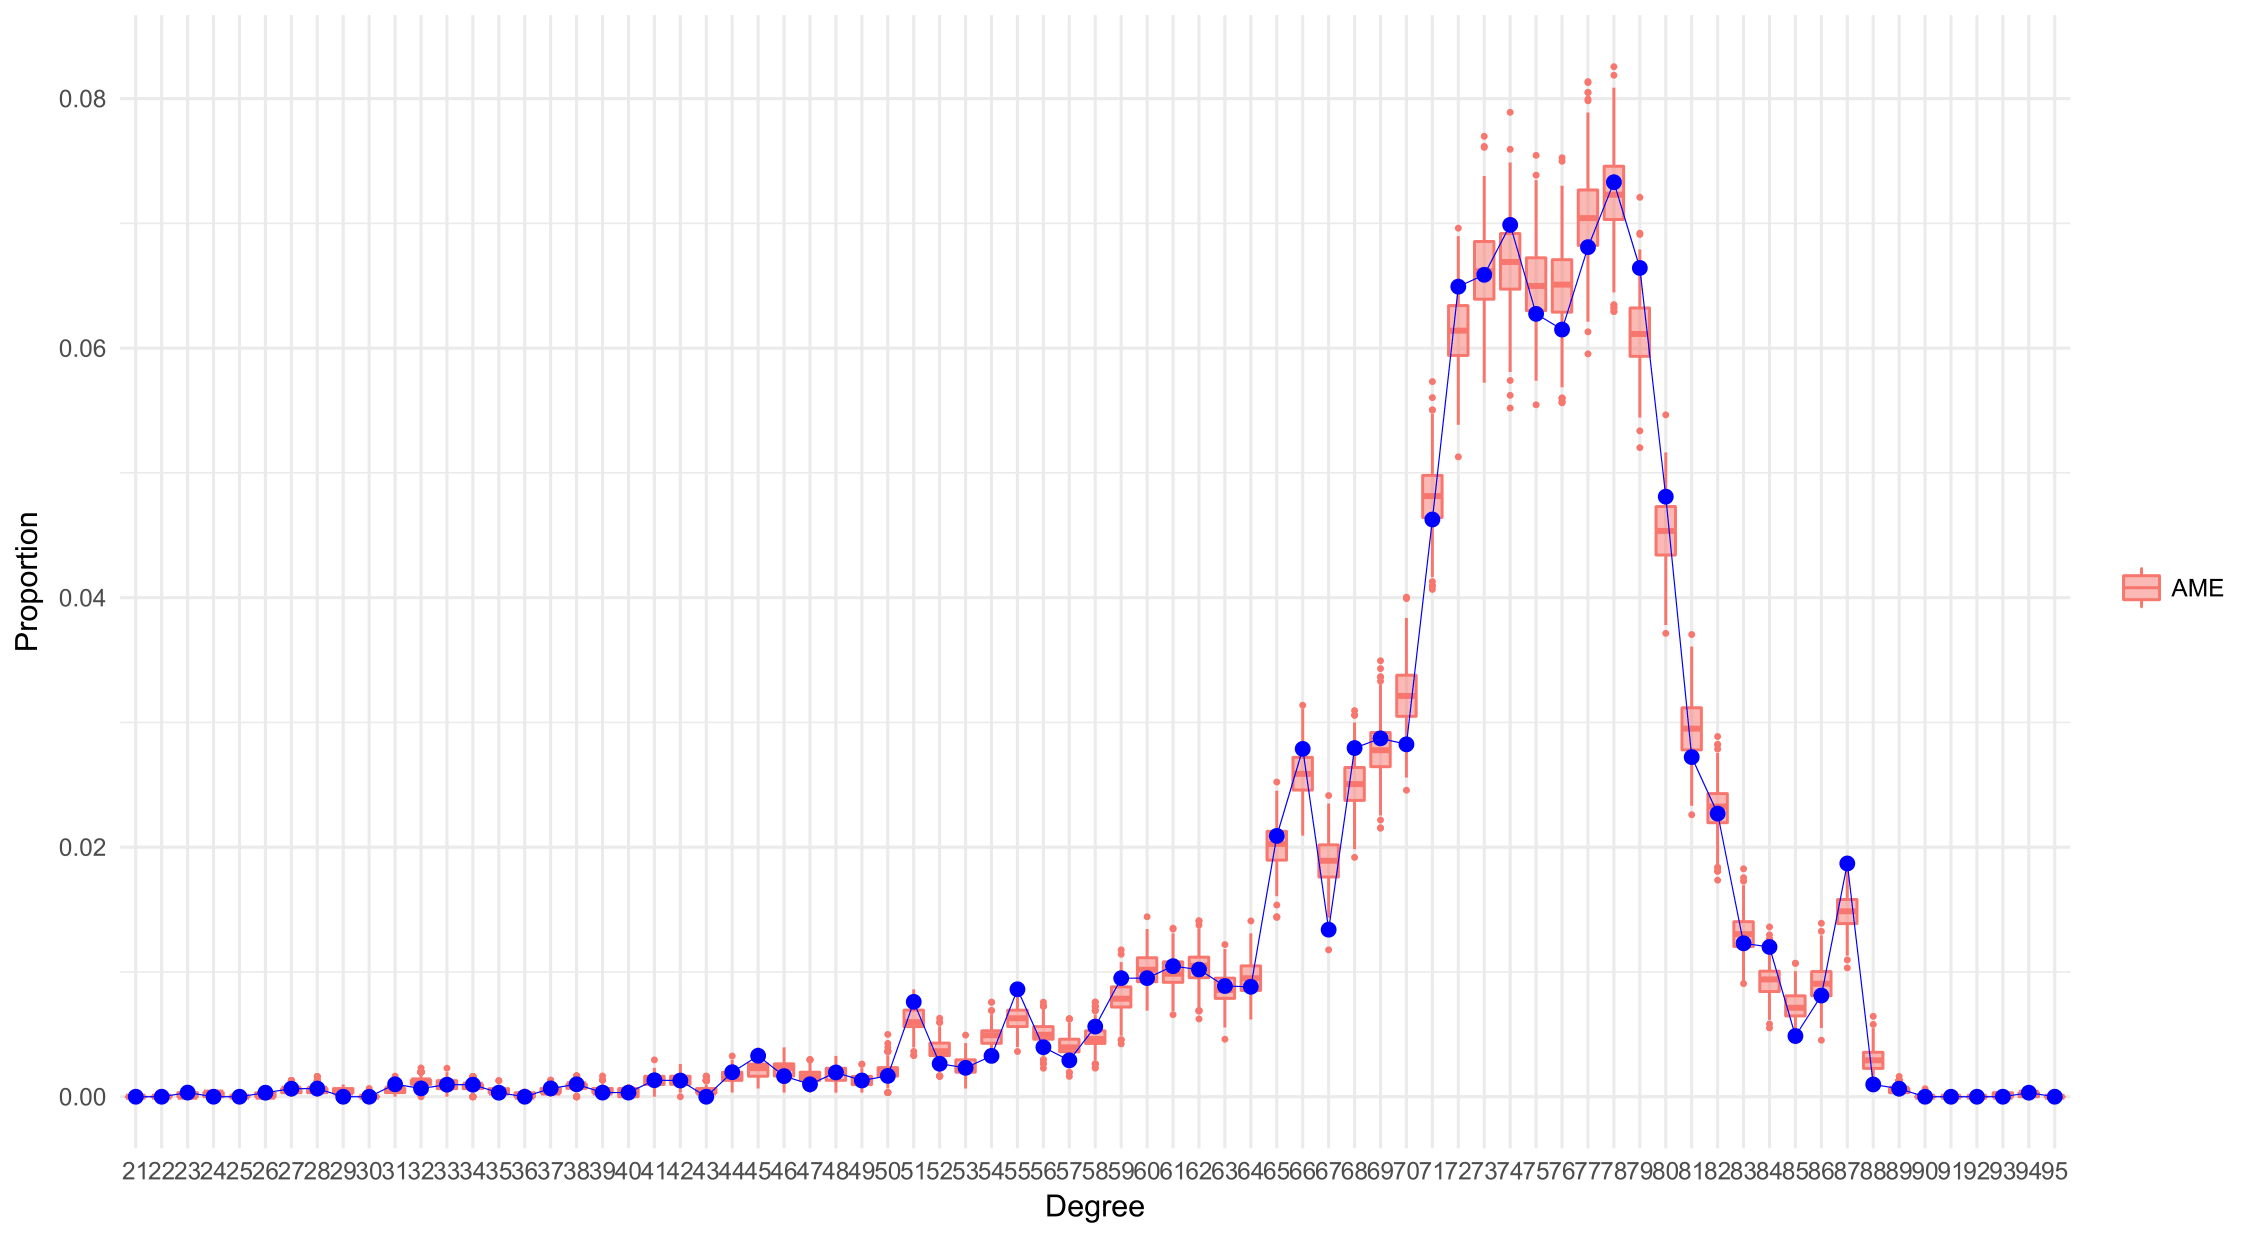
\includegraphics[width=0.85\textwidth]{plots_paper/AMEoveralldegree-1.png}	
			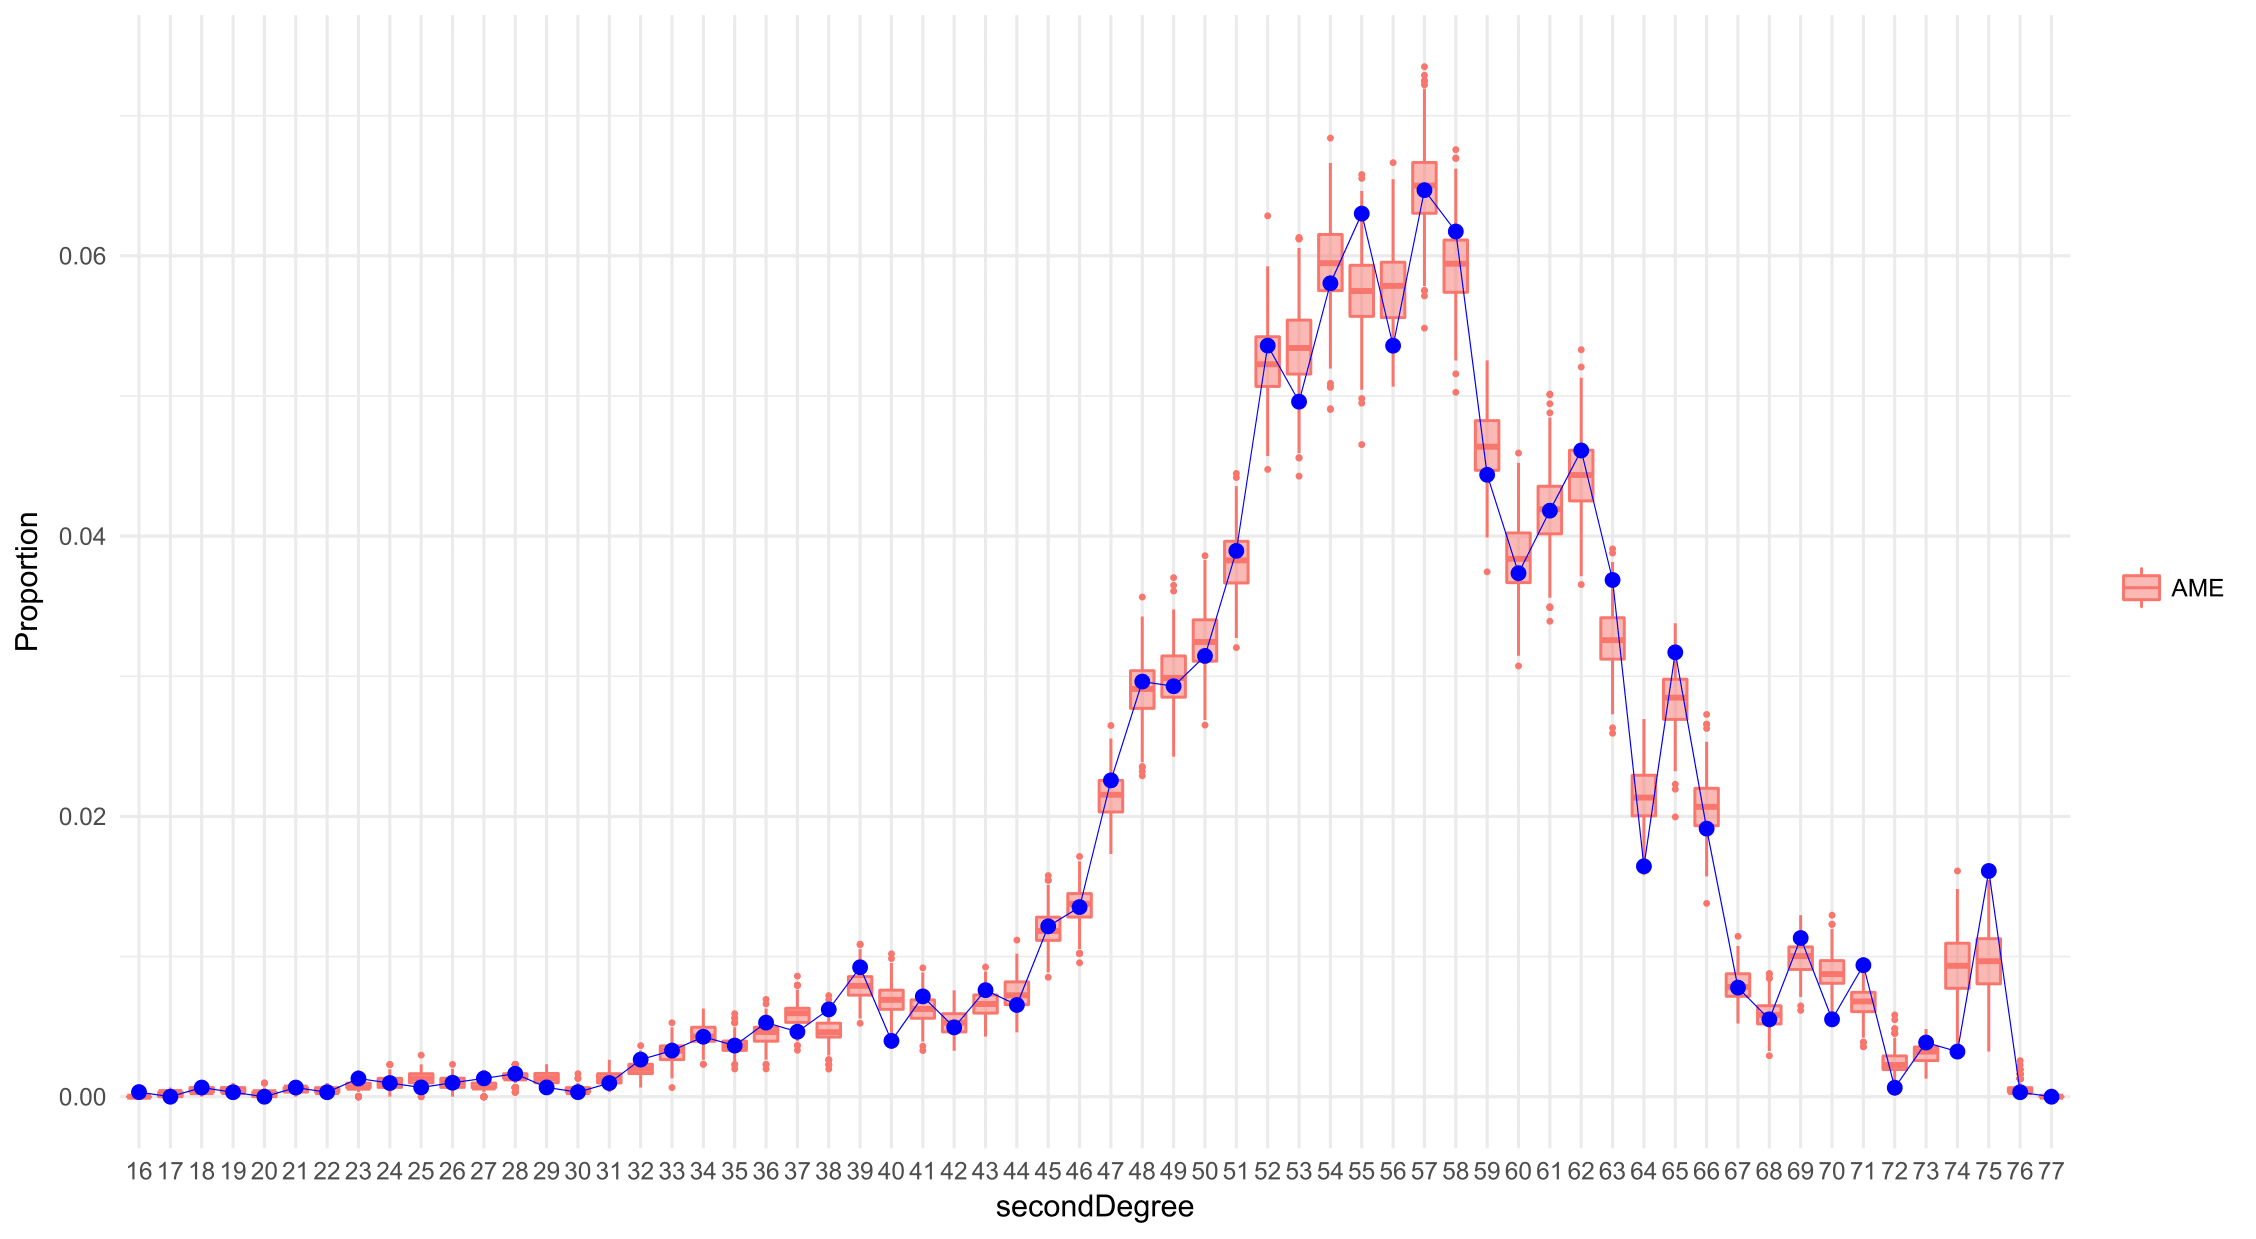
\includegraphics[width=0.85\textwidth]{plots_paper/AMEoverallsecond-1.png}	
				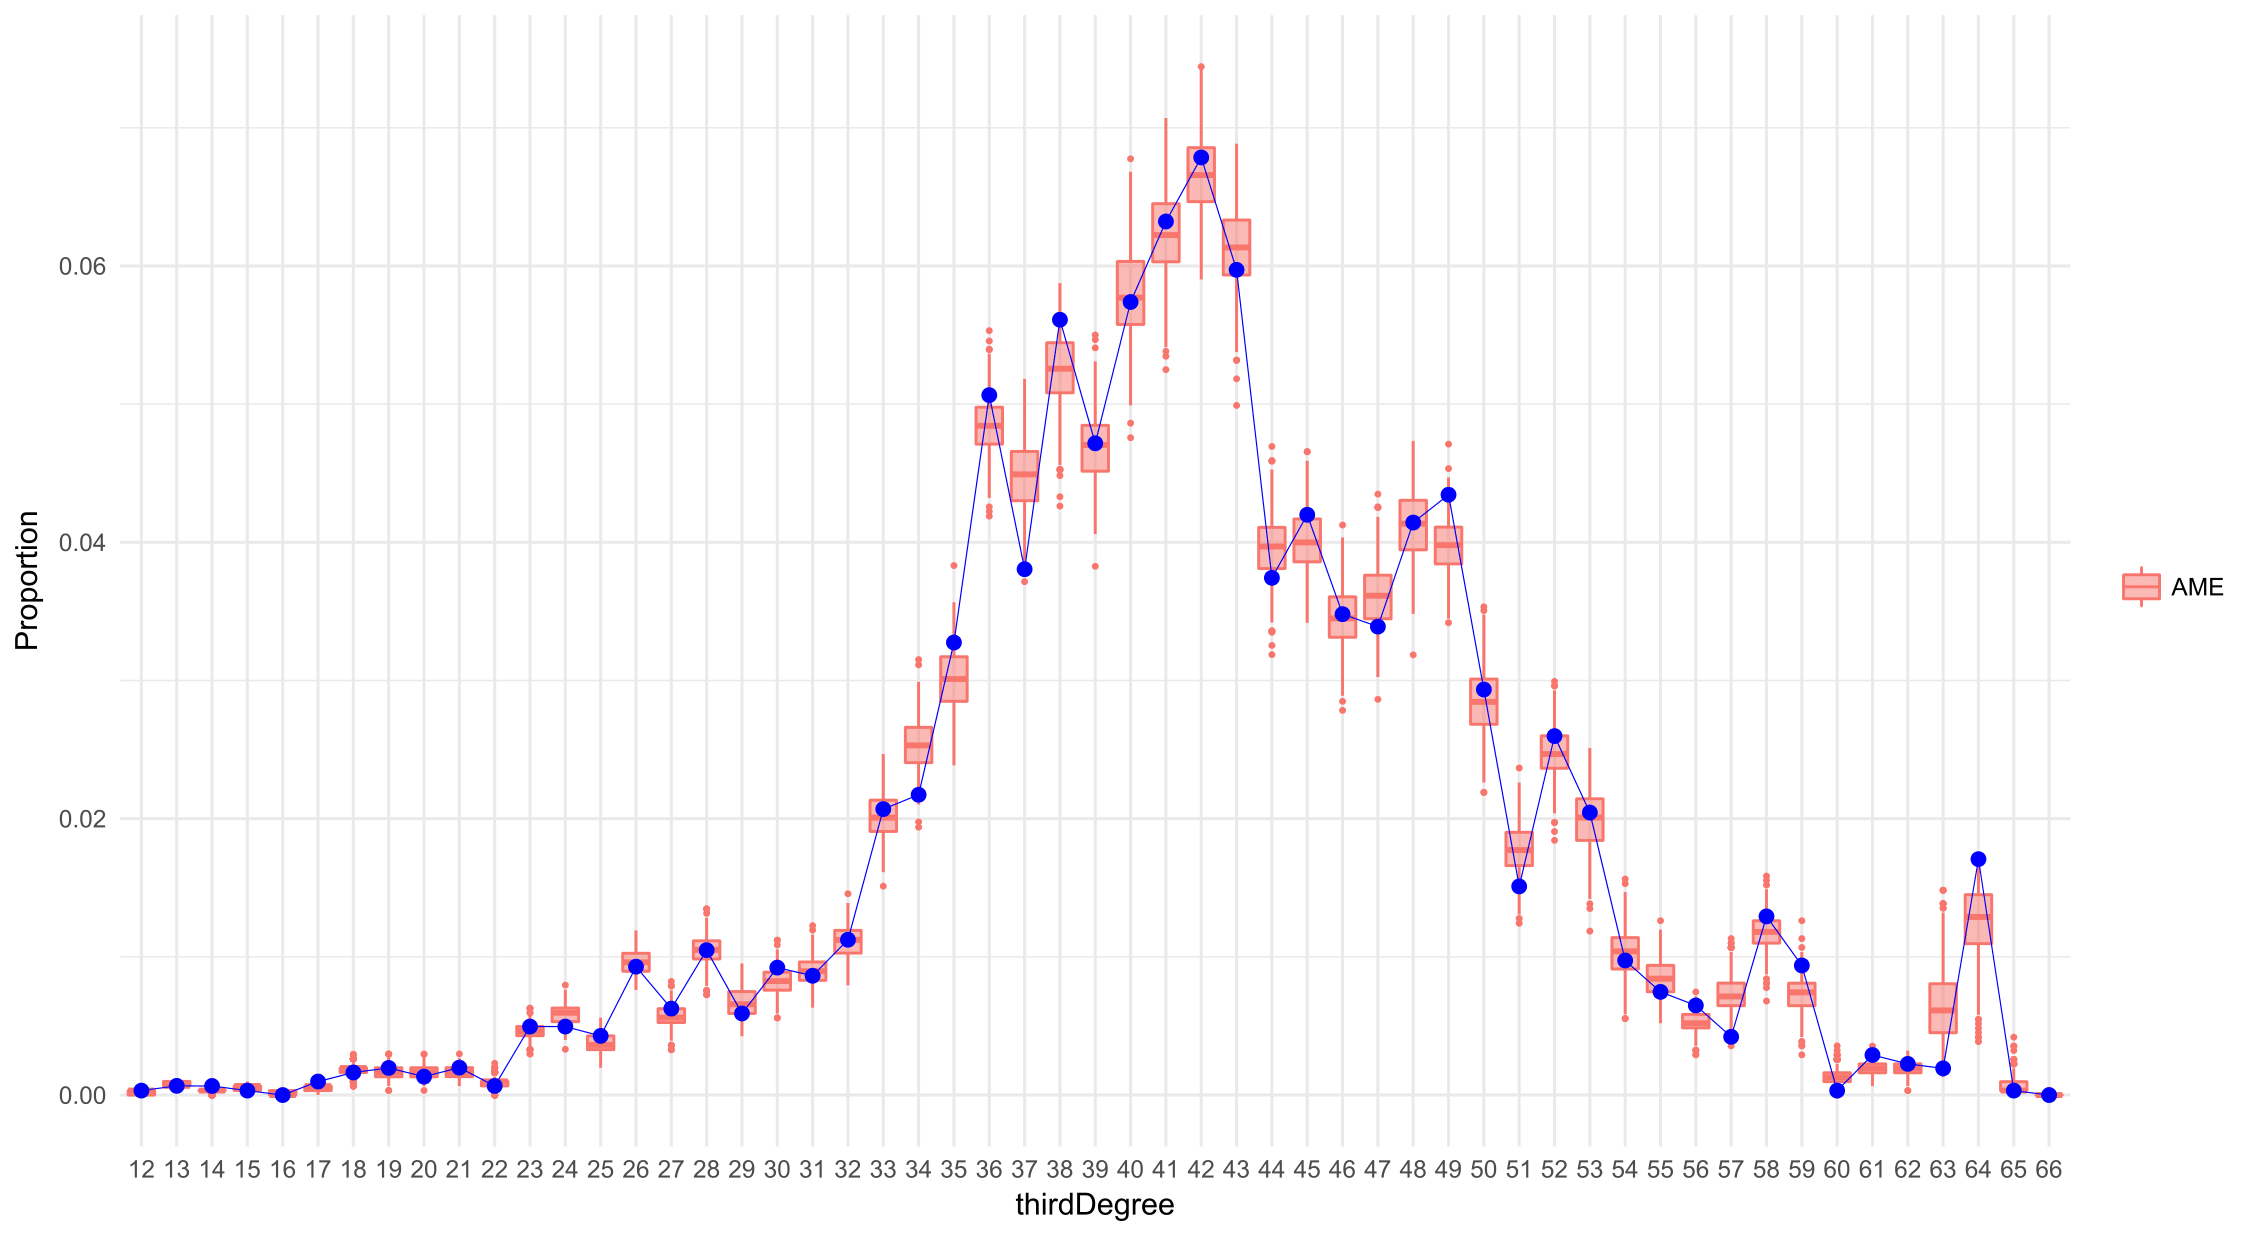
\includegraphics[width=0.85\textwidth]{plots_paper/AMEoverallthird-1.png}	
	\end{center}
\end{figure}

\end{appendices}
\end{document}

